With the methods and approaches developed in \autoref{chap:oneD} for the one-dimensional model, we have an expectation of the behavior of the two-dimensional Stommel model around the non-smooth bifurcation under similar conditions. With the bifurcation structure we explored in \autoref{chap:introduction}, we consider a generalization of the Stommel model with

\begin{equation}\label{eq:twoD_canonical}
  \begin{aligned}
   \dot{V} & =  \eta_1-\eta_2+\eta_3(T-V)-T-V|V|+A\sin(\Omega t), \\
   \dot{T}     & =  \eta_1-T(1+|V|)+B\sin(\Omega t),  \\
  \dot{\eta_2}  & =  -\epsilon\\
  V(0)=&V^0,\quad T(0)=T^0, \quad \eta_2(0)={\eta_2}^0>\eta_1\eta_3,
  \end{aligned}
\end{equation}

with slow variation $\epsilon\ll 1$, high frequency $\Omega\gg 1$, amplitudes of oscillation $A$ and $B$, and model parameters $\eta_1$ and $\eta_3$ as positive constants. We assume the initial conditions $V^0$, $T^0$ and $\eta_2^0$ are along the lower equilibrium branch which puts emphasis on the non-smooth behavior of the Stommel model with two additional features. First, we allow for slow variation in the bifurcation parameter which has been shown to be realistic since the $\eta_2$ is related to the freshwater flux and therefore not a fixed parameter; the same assumption is made in Roberts \cite{roberts2017relaxation}. Second, we consider periodic forcing in the additive parameters $\eta_1$ and $\eta_2$ to account for oscillations in the observed behavior in Huybers \cite{huybers2005obliquity}. To fully understand the effects of each component on the model, we consider them individually before putting them together.

For the remainder of this paper, we make two assumptions: first that $\eta_3<1$ locates the smooth bifurcation of \eqref{eq:twoD_canonical}  in the positive $V$ region. The value of $\eta_3$ describes the relative strength of the temperature relaxation to that of salinity, and it is frequently assumed that salinity has a slower relaxation, giving $\eta_3<1$. We restrict our attention to $\eta_3<1$, since the case of $\eta_3>1$ follows similarly. The second assumption we make is that even though we have a model in terms of $V$ and $T$, the variable $V$ is driving the dynamics of the system as confirmed in the analysis below. This assumption means that we want to understand the non-smooth behavior in $V$ where $T$ follows in response to the effects of $V$. The evidence below shows changes in temperature respond to changes in salinity. This assumption allows for a reduced model, expressing the behavior of $T$ in terms of $V$ to find equations in only one variable.

\section{Slowly Varying Bifurcation Parameter}
\label{sec:twoD_slow}

We consider the slow variation mechanism to understand the effects on the Stommel model \eqref{eq:twoD_canonical} with $\epsilon>0$ and $A=B=0$, where the bifurcation parameter $\eta_2$ slowly varies without oscillatory forcing. Then we expect to find a tipping point in the neighborhood of the aforementioned non-smooth bifurcation at $\eta_2=\eta_1\eta_3$. With the choice of $\eta_3<1$, the lower branch with $V<0$ is the branch we focus on in order to approach the non-smooth behavior, thus \eqref{eq:twoD_canonical} is

\begin{equation}\label{eq:twoD_slow_negative}
 \begin{aligned}
   \dot{V} & =  \eta_1-\eta_2(t)+\eta_3(T-V)-T+V^2, \\
   \dot{T} & =  \eta_1-T(1-V),  \\
  \dot{\eta_2}  & =  -\epsilon.
  \end{aligned}
\end{equation}

From \autoref{sec:oneD_slow}, we learned that the one-dimensional model had a solution that displayed one type of behavior away from the non-smooth $x=0$ and another type close to $x=0$ and a local analysis gave insight into the tipping. Here we search for an outer solution to \eqref{eq:twoD_slow_negative} that helps us understand the behavior of system away from the non-smooth $V=0$.  Since we have slow variation in $\eta_2$, we choose to scale the system \eqref{eq:twoD_slow_negative} with the 'slow' time $\tau=\epsilon t$

\begin{equation}\label{eq:twoD_slow_slowsystem}
\begin{aligned}
\epsilon V_\tau =&\eta_1-\eta_2(\tau)+\eta_3(T-V)-T+V^2, \\
\epsilon T_\tau & =  \eta_1-T(1-V),  \\
  {\eta_2}_\tau  & =  -1.
\end{aligned}
\end{equation}

We use asymptotic expansions in terms of the small quantity $\epsilon$ to look for slowly varying solutions. Here we choose

\begin{equation}\label{eq:twoD_slow_outerexpansion}
\begin{aligned}
V(\tau)\sim &V_0(\tau)+\epsilon V_1(\tau)+\epsilon^2 V_2(\tau)+\ldots\\
T(\tau)\sim & T_0(\tau)+\epsilon T_1(\tau)+\epsilon^2 T_2(\tau)+\ldots
\end{aligned}
\end{equation}

and substitute \eqref{eq:twoD_slow_outerexpansion} into \eqref{eq:twoD_slow_slowsystem} to find

\begin{equation*}
\begin{aligned}
 \epsilon{V_0}_\tau+\epsilon^2{V_1}_\tau+\ldots =&\begin{aligned}[t]
\eta_1-&\eta_2(\tau)+\eta_3(T_0-V_0)-T_0+V_0^2\\
&+\epsilon(\eta_3(T_1-V_1)-T_1-2V_1V_0)+\ldots
\end{aligned}\\
\epsilon{T_0}_\tau+\epsilon^2{T_1}_\tau+\ldots=&\eta_1-T_0(1-V_0)+\epsilon(-T_1(1-V_0)+V_1T_0)+\ldots
\end{aligned}
\end{equation*}

Here we separate at each order of $\epsilon$ to find the following system of equations

\begin{align}
\label{eq:twoD_slow_outerO1}
O(1):\quad & \begin{cases}
	0 =& \eta_1-\eta_2(\tau)+\eta_3(T_0-V_0)-T_0+V_0^2 , \\
	0 =&  \eta_1-T_0(1-V_0),\\
\end{cases}\\
\label{eq:twoD_slow_outerO2}
O(\epsilon):\quad & \begin{cases}
	{V_0}_\tau = & \eta_3(T_1-V_1)-T_1+2V_1V_0,\\
	{T_0}_\tau =&  -T_1(1-V_0)+V_1T_0,
\end{cases}
\end{align}

We then solve \eqref{eq:twoD_slow_outerO1} simultaneously for the pseudo-equilibria noting that $T_0$ is explicitly in terms of $V_0$ 

\begin{equation}\label{eq:twoD_slow_equilibria}
\begin{aligned}
T_0(V_0)=&\frac{\eta_1}{1-V_0},\\
0=\eta_1-\eta_2(\tau)-T_0(V_0)&+\eta_3(T_0(V_0)-V_0)+V_0^2.
\end{aligned}
\end{equation}

With $T_0$ and $V_0$ found, we solve \eqref{eq:twoD_slow_outerO2} for $T_1$ explicitly in terms of $V_1$ 

\begin{equation}\label{eq:twoD_slow_equilcorrec}
\begin{aligned}
&T_1(V_1) = \frac{{T_0}_\tau-T_0(V_0)V_1}{1-V_0},\\
V_1 =& \frac{-(1-V_0){V_0}_\tau+(1-\eta_3){T_0}_\tau({V_0}_\tau)}{(1-\eta_3)T_0(V_0)+(\eta_3-2V_0)(1-V_0)}.
\end{aligned}
\end{equation}

This gives the first few terms of the asymptotic expansion \eqref{eq:twoD_slow_outerexpansion} with \eqref{eq:twoD_slow_equilibria} and \eqref{eq:twoD_slow_equilcorrec}. Given these expressions, it is not immediately obvious in the two-dimensional problem when the outer solution breaks down. However, noting that for $V_0\to 0$ the asymptotic expansion for $V$ is no longer valid, we rescale the system to find an inner equation in this region. 

Analogous to \autoref{sec:oneD_slow}, this corresponds to the non-smooth bifurcation at $\eta_2=\eta_1\eta_3$ when $V=0$ and $T=\eta_1$, so it makes the most sense to rescale \eqref{eq:twoD_canonical} around these values. This results in the rescaled variables

\begin{equation}\label{eq:twoD_slow_rescale}
\begin{aligned}
\eta_2=&\eta_1\eta_3+\epsilon n,\\
V=&\epsilon X,\\
T=&\eta_1+\epsilon Y.
\end{aligned}
\end{equation}

Then we introduce these local variables \eqref{eq:twoD_slow_rescale} into the canonical system \eqref{eq:twoD_canonical} to find the following inner system

\begin{equation}\label{eq:twoD_slow_inner}
\begin{aligned}
   \dot{X} & =  -n(t)-\eta_3 X-(1-\eta_3)Y-\epsilon X|X|, \\
   \dot{Y} & =  -\eta_1 |X|-Y-\epsilon |X|Y,  \\
  \dot{n}  & =  -1.
  \end{aligned}
\end{equation}

We outline the influence of the parameters $\eta_1$ and $\eta_3$ on the behavior of a solution. We already determined from the introduction that $\eta_3$ determines the orientation of the problem, but here we find a relationship between the parameters $\eta_1$ and $\eta_3$ by viewing \eqref{eq:twoD_slow_inner} as a $2\times 2$ system of spatial coordinates and linearizing. This results in 

\begin{equation}\label{eq:twoD_slow_innermatrix}
\begin{pmatrix}
\dot{X}\\
\dot{Y}
\end{pmatrix}=
\begin{pmatrix}
-\eta_3 & -(1-\eta_3) \\ 
-\eta_1\text{sgn}(X) & -1
\end{pmatrix}
\begin{pmatrix}
X\\
Y
\end{pmatrix}-
\begin{pmatrix}
n(t)\\
0
\end{pmatrix}.
\end{equation}

Here a linearized stability analysis about the pseudo-equilibria similar to \cite{seydel2009practical} is needed to determine the stability of the lower pseudo-equilibria. This is performed in Dijkstra \cite{dijkstra2013nonlinear} and hence we note that both stability of the lower branch and non-hyperbolic behavior at $({\eta_2}_{ns},V_{ns})=(\eta_1\eta_3,0)$ is observed. Thus we expect our tipping point to occur just after the standard non-smooth bifurcation. With this in mind, we consider $V>0$ and with \eqref{eq:twoD_slow_innermatrix} we find the inner system

\begin{equation}\label{eq:twoD_slow_positiveinner}
 \begin{aligned}
   \dot{X} & =  -n(t)-\eta_3 X-(1-\eta_3)Y-\epsilon X^2, \\
   \dot{Y} & =  -\eta_1 X-Y-\epsilon XY,  \\
  \dot{n}  & =  -1.
  \end{aligned}
\end{equation}

Following the approach from \autoref{sec:oneD_slow}, we change the differentiation to be in terms of $n$ to find

\begin{equation*}
\begin{pmatrix}
X_n\\
Y_n
\end{pmatrix}=
\begin{pmatrix}
\eta_3 & 1-\eta_3 \\ 
\eta_1 & 1
\end{pmatrix}
\begin{pmatrix}
X\\
Y
\end{pmatrix} +
\begin{pmatrix}
n+\epsilon X^2\\
\epsilon XY
\end{pmatrix}.
\end{equation*}

Seeking a leading order solution in this region, we drop the $\epsilon$ order terms to give 

\begin{equation}\label{eq:twoD_slow_uppermatrix}
\begin{pmatrix}
X_n\\
Y_n
\end{pmatrix}=
\begin{pmatrix}
\eta_3 & 1-\eta_3 \\ 
\eta_1 & 1
\end{pmatrix}
\begin{pmatrix}
X\\
Y
\end{pmatrix} +
\begin{pmatrix}
n\\
0
\end{pmatrix}.
\end{equation}

For the system \eqref{eq:twoD_slow_uppermatrix}, we find the following eigenvalues using \eqref{eq:twoD_slow_eigen}

\begin{equation}\label{eq:twoD_slow_uppereigen}
\lambda_{1,2}=\frac{\eta_3+1}{2}\pm\frac{1}{2}\sqrt{(1+\eta_3)^2+4(\eta_1(1-\eta_3)-\eta_3)}.
\end{equation}

These eigenvalues in \eqref{eq:twoD_slow_uppereigen} must be real as $\eta_3<1$ guarantees the discriminant is always positive. But the stability also follows as one of the eigenvalues is positive and the other is negative. This causes the solution to be unstable, which confirms tipping to occur in the region $V>0$. With real eigenvalues, the solution in the $V>0$ region takes the following exponential form with constants $K_{i,j}$ being component $j$ of the corresponding $i$ eigenvector 

\begin{equation}\label{eq:twoD_slow_innersoln}
\begin{aligned}
X(n)\sim& K_{1,1}e^{\lambda_1 n}+K_{2,1}e^{\lambda_2 n}+C_1 n+C_2,\\
Y(n)\sim& K_{1,2}e^{\lambda_1 n}+K_{2,2}e^{\lambda_2 n}+C_3 n+C_4.\\
\end{aligned}
\end{equation}

Translating both solutions in \eqref{eq:twoD_slow_inner} back to our original coordinates we find

\begin{equation}\label{eq:twoD_slow_inneroriginal}
\begin{aligned}
V(t)\sim&  \epsilon K_{1,1}e^{\lambda_1(\eta_2(t)-\eta_1\eta_3)/\epsilon}+\epsilon K_{2,1}e^{\lambda_1(\eta_2(t)-\eta_1\eta_3)/\epsilon}+O(\epsilon),\\
T(t)\sim& \eta_1+ \epsilon K_{1,2}e^{\lambda_1 (\eta_2(t)-\eta_1\eta_3)/\epsilon}+\epsilon K_{2,2}e^{\lambda_2 (\eta_2(t)-\eta_1\eta_3)/\epsilon}+O(\epsilon).
\end{aligned}
\end{equation}

With \eqref{eq:twoD_slow_inneroriginal} admitting the solution in the region $V>0$, we determine the system to tip once one of these exponentials becomes large (i.e $O(1/\epsilon)$), which causes the system to diverge away from our lower branch towards the upper stable branch. Thus the tipping point ${\eta_2}_{\text{slow}}$ is

\begin{equation}\label{eq:twoD_slow_tipping}
{\eta_2}_{\text{slow}}= \min\limits_i\{\eta_1\eta_3-\epsilon\ln\epsilon/\lambda_i\},\quad i=1,2.
\end{equation}

Thus we have the tipping for this problem with \eqref{eq:twoD_slow_tipping} and this has a similar form to the tipping point from \autoref{sec:oneD_slow}. As we found from \eqref{eq:twoD_slow_uppereigen}, one of the eigenvalues is always positive and it is with this we find that the tipping point is less than the bifurcation. This means the slow variation causes a delay in the rapid transition from the lower branch to the upper branch and the solution spends more time around the lower branch. These effects shrink as $\epsilon\to 0$ until we return to the static problem with $\epsilon=0$,

\begin{figure}[H]
\centering
\begin{subfigure}{.5\textwidth}
  \centering
  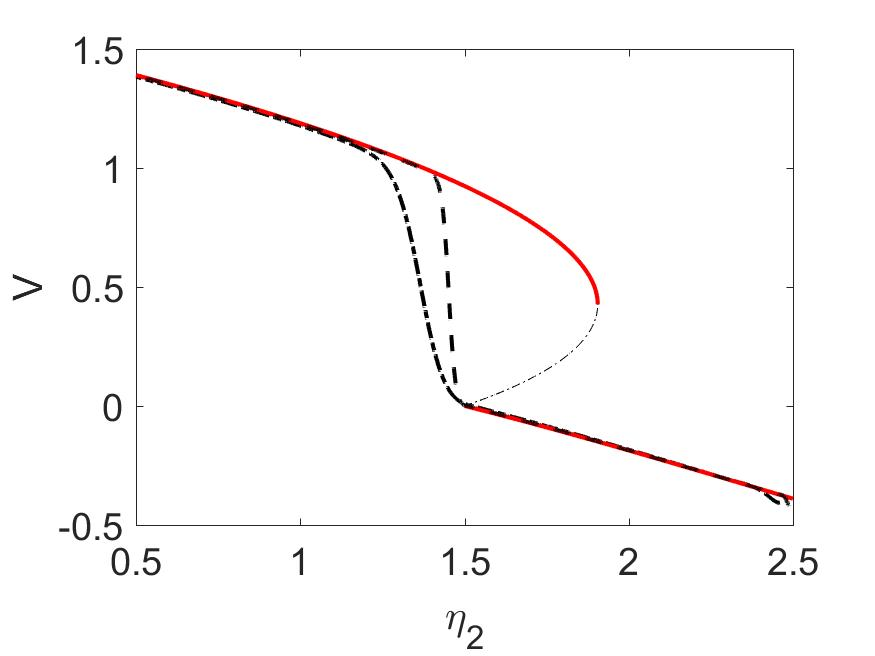
\includegraphics[width=\linewidth]{twoD/slow_bif_diagram.jpg}
  \caption{}
\end{subfigure}%
\begin{subfigure}{.5\textwidth}
  \centering
  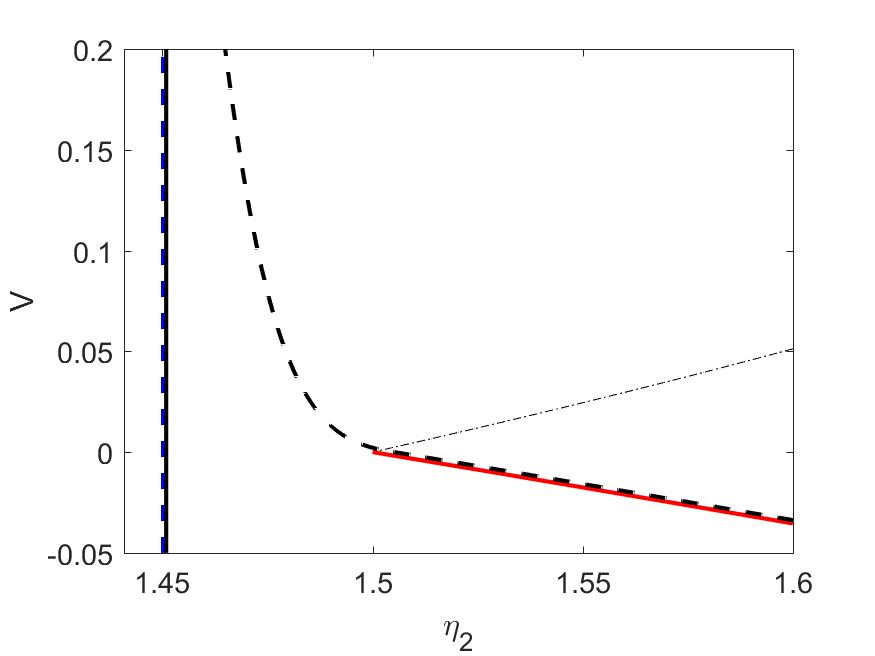
\includegraphics[width=\linewidth]{twoD/slow_bif_diagram_zoom.jpg}
  \caption{}
\end{subfigure}
\caption{In (a) the numerical solution (black dotted line) to \eqref{eq:twoD_canonical} is given with $\eta_1=4$, $\eta_3=.375$, and $\epsilon=.01$. In (b) a zoom in closer to the non-smooth bifurcation region where the blue dotted vertical line is the prediction \eqref{eq:twoD_slow_tipping} against the black solid vertical line which is the numerical tipping point.}
\label{fig:twoD_slow_Vnumerics}
\end{figure}

In figure~\ref{fig:twoD_slow_Vnumerics} an example of a slowly varying $\eta_2$ is given for a choice of $\epsilon$ in (a) and we zoom in around the non-smooth bifurcation in (b). Here we use the tipping criteria to be whenever $V>0.5$, this is large enough that the solution is strongly moving towards the upper branch and is around the point of the smooth bifurcation. The delay in moving towards the upper branch in the $V$ solution causes a similar delay in $T$ seen in figure~\ref{fig:twoD_slow_Tnumerics}. This is best explained in the perturbation equation \eqref{eq:twoD_slow_pertub} where the solution is attracted to below the pseudo-equilibrium. Thus when the tipping point in $V$ is reached, the solution for $T$ has yet to reach the maximum value. Here notice that after the tipping occurs, the numerical solution passes entirely over the unstable branch and even some of the upper stable branch before following the upper branch closely.

\begin{figure}[H]
\centering
\begin{subfigure}{.5\textwidth}
  \centering
  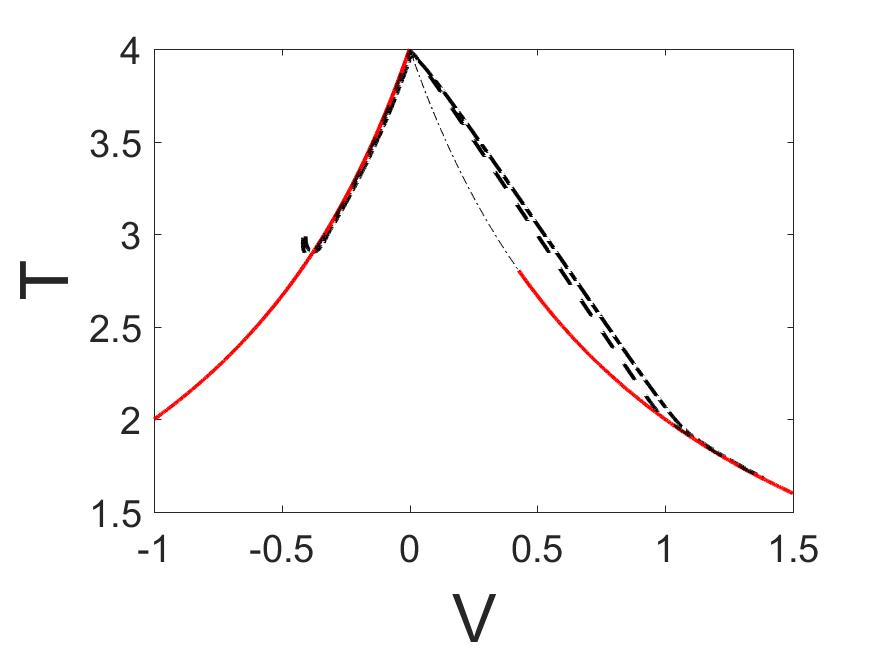
\includegraphics[width=\linewidth]{twoD/slow_bif_Tplot.jpg}
  \caption{}
\end{subfigure}%
\begin{subfigure}{.5\textwidth}
  \centering
  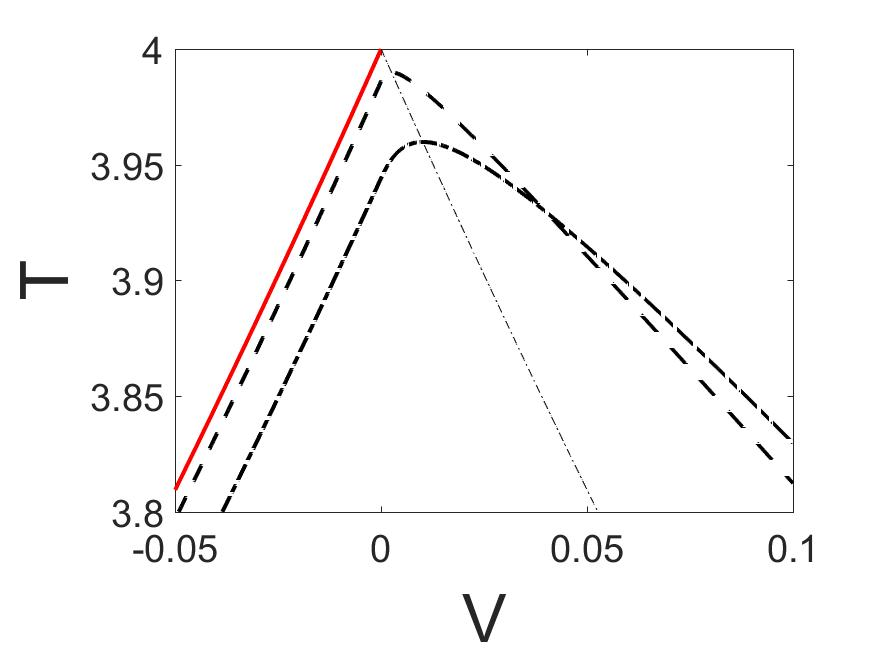
\includegraphics[width=\linewidth]{twoD/slow_bif_Tplot_zoom.jpg}
  \caption{}
\end{subfigure}
\caption{In (a) we have the numerical solution (black dotted) over the standard equilibrium plot for $V$ vs. $T$. In (b) a zoom of the bifurcation area.}
\label{fig:twoD_slow_Tnumerics}
\end{figure}

In figure~\ref{fig:twoD_slow_epscomp} we compare the numerical tipping to the predicted tipping in \eqref{eq:twoD_slow_tipping} over a range of $\epsilon$. Here we see performance even better than in section \autoref{sec:oneD_slow} as even for relatively large $\epsilon$ the prediction has small error. This is an artifact of having a higher dimensional problem, where now two exponentials in \eqref{eq:twoD_slow_inneroriginal} are dominating the behavior of the solution in the $V>0$ region. As in \autoref{sec:oneD_slow}, the concavity of the predicted tipping against the numerical tipping match very well and we can expect the prediction to hold for reasonably small values of $\epsilon$.

\begin{figure}[H]
\centering
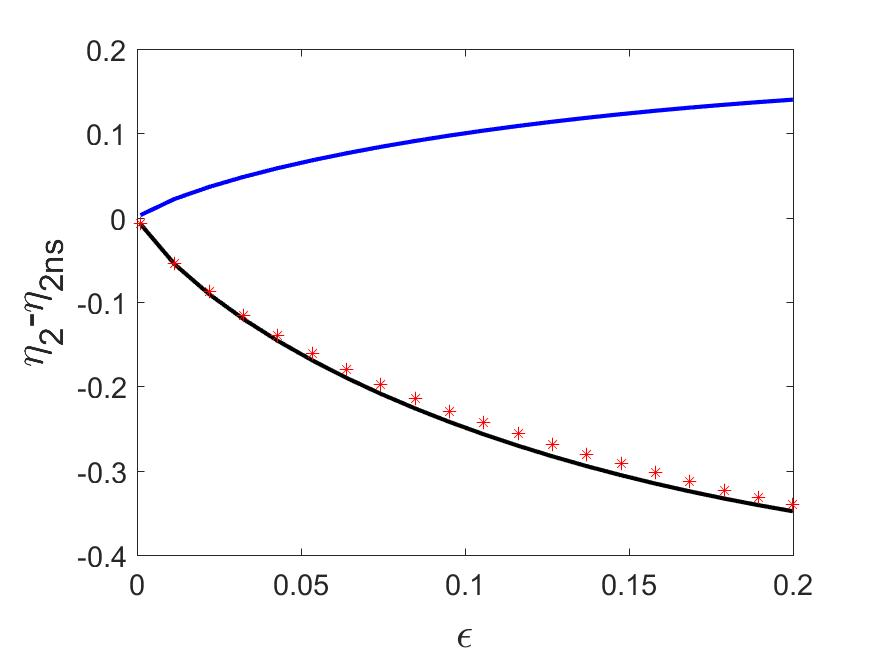
\includegraphics[width=\linewidth]{twoD/slow_epscomp.jpg}
\caption{The numerical tipping vs the estimate with $\eta_1=4$ and $\eta_3=\frac{3}{8}$, where ${\eta_2}_{\text{ns}}=\eta_1\eta_3$. The top blue line is the tipping of the second eigenvalue. The tipping criteria is $V>.5$.}
\label{fig:twoD_slow_epscomp}
\end{figure}

\section{High Frequency Oscillatory Forcing}
\label{sec:twoD_highfreqosc}

We consider oscillations occurring in the dynamics that is not originally encompassed by the Stommel model \cite{alley2003abrupt,huybers2005obliquity,marotzke2000abrupt,rahmstorf2000thermohaline,rahmstorf2002ocean,stastna2007box}. We choose to allow $\eta_1$ and $\eta_2$ to exhibit oscillatory behavior to account for this. As these parameters appear in both equations for $V$ and $T$, here we consider the canonical system \eqref{eq:twoD_canonical} with $A,B\sim O(1)$, $\Omega\gg 1$ and $\epsilon=0$ which is the purely oscillatory forcing problem. Under these conditions, like in the one-dimensional model in \autoref{sec:oneD_highfreqosc}, we expect to find oscillations that are attracting; this stable behavior should act like oscillations about the equilibria of a reduced inner problem. Thus our analysis must locate these equilibria as a function of $\eta_2$ in order to find the bifurcation.

To begin our analysis, we note that the dynamics occur on multiple time scales, a 'slow' $t$ and 'fast' $R = \Omega t$. Following the multiple scales method, we consider $V(t)=V(t,R)$ and $T(t)=T(t,R)$ and substituting this into \eqref{eq:twoD_canonical}, we get the system

\begin{equation}\label{eq:twoD_osc_multiscaleouter}
\begin{aligned}
V_R+\Omega^{-1}V_t = & \Omega^{-1}\left(\eta_1-\eta_2+\eta_3(T-V)-T-V|V|+A\sin(R)\right),\\
T_R+\Omega^{-1}T_t = & \Omega^{-1}\left(\eta_1-T(1+|V|)+B\sin(R)\right).
\end{aligned}
\end{equation}

We follow the lower branch to study dynamics near the non-smooth bifurcation. Thus we consider the system \eqref{eq:twoD_osc_multiscaleouter} with $V<0$

\begin{equation}\label{eq:twoD_osc_multiscaleouterlower}
\begin{aligned}
V_R+\Omega^{-1}V_t = & \Omega^{-1}\left(\eta_1-\eta_2+\eta_3(T-V)-T+V^2+A\sin(R)\right),\\
T_R+\Omega^{-1}T_t = & \Omega^{-1}\left(\eta_1-T(1-V)+B\sin(R)\right).
\end{aligned}
\end{equation}

From \eqref{eq:twoD_osc_multiscaleouterlower}, it makes sense to consider an asymptotic expansion for both $V$ and $T$ in terms of the small quantity that appears, $\Omega^{-1}$, with

\begin{equation}\label{eq:twoD_osc_outerexpansion}
\begin{aligned}
V(t,R)\sim V_0(t,R) +\Omega^{-1}V_1(t,R) +\Omega^{-2}V_2(t,R)+O(\Omega^{-3}),\\
T(t,R)\sim T_0(t,R) +\Omega^{-1}T_1(t,R) +\Omega^{-2}T_2(t,R)+O(\Omega^{-3}).
\end{aligned}
\end{equation}

Substituting \eqref{eq:twoD_osc_outerexpansion} into the system \eqref{eq:twoD_osc_multiscaleouterlower} gives

\begin{equation*}
\begin{aligned}
{V_0}_R+\Omega^{-1}{V_0}_t+\Omega^{-1}{V_1}_R+\ldots=&\begin{aligned}[t]\Omega^{-1}&(\eta_1-\eta_2+\eta_3(T_0-V_0)-T_0+V_0^2+A\sin(R))\\
+&\Omega^{-2}(\eta_3(T_1-V_1)-T_1+2V_1V_0)+\ldots
\end{aligned}\\
{T_0}_R+\Omega^{-1}{T_0}_t+\Omega^{-1}{T_1}_R+\ldots=&\begin{aligned}[t]  \Omega^{-1}&(\eta_1-T_0(1-V_0)+B\sin(R))\\
+&\Omega^{-2}(-T_1(1-V_0)+T_0V_1)+\ldots
\end{aligned}
\end{aligned}
\end{equation*}

Here we find the following equations separated by order of $\Omega^{-1}$ with

\begin{align}
\label{eq:twoD_osc_outerO1}
O(1):\quad & \begin{cases}
	{V_0}_R =&  0, \\
	{T_0}_R =&  0,\\
\end{cases}\\
\label{eq:twoD_osc_outerO2}
O(\Omega^{-1}):\quad & \begin{cases}
	{V_1}_R+{V_0}_t = & \eta_1-\eta_2+\eta_3(T_0-V_0)-T_0+V_0^2+A\sin(R),\\
	 {T_1}_R +{T_0}_t =&  \eta_1-T_0(1-V_0)+B\sin(R),
\end{cases}\\
\label{eq:twoD_osc_outerO3}
O(\Omega^{-2}):\quad & \begin{cases}
	{V_2}_R+{V_1}_t = & \eta_3(T_1-V_1)-T_1+2V_0V_1,\\
	 {T_2}_R +{T_1}_t =&  -T_1(1-V_0)+T_0V_1.
\end{cases}
\end{align}

We learn from \eqref{eq:twoD_osc_outerO1} that both our leading order terms are purely dependent on the slow variable, $V_0=V_0(t)$, $T_0=T_0(t)$. But much like \autoref{sec:oneD_highfreqosc}, we must introduce a solvability condition on the resonant terms to be able to solve for the correction terms, ensuring for the sub-linear growth resulting in a stable solution. Here, we use the Fredholm alternative \eqref{eq:Fredholm} on \eqref{eq:twoD_osc_outerO2}-\eqref{eq:twoD_osc_outerO3} and search for the equilibrium solutions, this is shown in \autoref{app:twoD}. This leads to the outer solution in original coordinates

\begin{equation}\label{eq:twoD_osc_outersoln}
\begin{aligned}
V\sim& V_0-\Omega^{-1} A\cos(\Omega t)+\dots\\
%\Omega^{-2}\left(V_2(t)+\left(A(\eta_3-2V_0)+B(1-\eta_3)\right)\sin(\Omega t)\right),\\
T\sim& T_0-\Omega^{-1} B\cos(\Omega t)+\ldots%\Omega^{-2}\left(T_2(t)+(1-V_0)B-T_0A)\sin(\Omega t)\right).
\end{aligned}
\end{equation}

Here both $V_0$ and $T_0$ are the same equilibrium solutions from the static model in the introduction with

\begin{equation*} \label{eq:twoD_lowerleadingorder}
\begin{aligned}
T_0(V_0)=&\frac{\eta_1}{1-V_0},\\
0=\eta_1-\eta_2+\eta_3&(T_0(V_0)-V_0)-T_0(V_0)+V_0^2.
\end{aligned}
\end{equation*}

For the one-dimensional model in \autoref{sec:oneD_highfreqosc}, we had to use a local expansion so we needed to scale both the coordinate $x$ as well as the parameter $\mu$ and analyze the local behavior around the axis $x=0$. Since we again have non-smooth dynamics at the axis $V=0$, we expect to use a local expansion for the two-dimensional model as well. While the precise scaling of the breakdown of the outer solution \eqref{eq:twoD_osc_outersoln} is too complex for us to search for, we instead observe that once $V_0$ becomes small the oscillations begin to dominate the solution and this is not consisten with our assumptions of the expansion. So we introduce a rescaling analogous to  \autoref{sec:oneD_highfreqosc}

\begin{equation}\label{eq:twoD_osc_scales}
\begin{aligned}
V=&\Omega^{-1}X,\\
T=& \eta_1 +\Omega^{-1}Y,\\
\eta_2=&\eta_1\eta_3+\Omega^{-1} n.
\end{aligned}
\end{equation}

Substituting \eqref{eq:twoD_osc_scales} into \eqref{eq:twoD_canonical} leads to the following inner system

\begin{equation}\label{eq:twoD_osc_innersystem}
\begin{aligned}
\dot{X}=& -n+\eta_3(Y-X)-Y-\Omega^{-1}X|X| +\Omega A\sin(\Omega t),\\
\dot{Y}=& -\eta_1|X|-Y -\Omega^{-1}|X|Y +\Omega A \sin(\Omega t).
\end{aligned}
\end{equation}

The form suggests behavior on the same time scales in \eqref{eq:twoD_osc_innersystem}, the 'slow' $t$ and the 'fast' $R=\Omega t$. Considering $X(t)=X(t,R)$ and $Y(t)=Y(t,R)$ gives the multiple scales inner system

\begin{equation}\label{eq:twoD_osc_innermulti}
\begin{aligned}
X_R+\Omega^{-1}X_t =& \Omega^{-1}\left(-n +\eta_3(Y-X)-Y\right)-\Omega^{-2}X|X|+A\sin(R),\\
Y_R+\Omega^{-1}Y_t =& \Omega^{-1}\left(-\eta_1|X|-Y\right)-\Omega^{-2}|X|Y+ B\sin(R).
\end{aligned}
\end{equation}

Once more, as we see the small quantity $\Omega^{-1}$ appearing in \eqref{eq:twoD_osc_innermulti}, we choose an expansion of the form

\begin{equation}\label{eq:twoD_osc_innerexpan}
\begin{aligned}
X(t,R)\sim& X_0(t,R)+\Omega^{-1}X_1(t,R)+O(\Omega^{-2}),\\
Y(t,R)\sim& Y_0(t,R)+\Omega^{-1}Y_1(t,R)+O(\Omega^{-2}),
\end{aligned}
\end{equation}

where we then substitute \eqref{eq:twoD_osc_innerexpan} into \eqref{eq:twoD_osc_innermulti} to give

\begin{equation*}
\begin{aligned}
{X_0}_R+\Omega^{-1}{X_0}_t+\Omega^{-1}{X_1}_R+\ldots=&\begin{aligned}[t]\Omega^{-1}&(-n+\eta_3(Y_0-X_0)-Y_0)+A\sin(R)\\
+&\Omega^{-2}(X_0|X_0+\Omega^{-1}X_1+\ldots|+\eta_3(Y_1-X_1)-Y_1)+\ldots
\end{aligned}\\
{Y_0}_R+\Omega^{-1}{Y_0}_t+\Omega^{-1}{Y_1}_R+\ldots=&\begin{aligned}[t]\Omega^{-1}&(-\eta_1|X_0+\Omega^{-1}X_1+\ldots|-Y_0)+B\sin(R)\\
+&\Omega^{-2}(-|X_0+\Omega^{-1}X_1+\ldots|Y_0-Y_1)+\ldots
\end{aligned}
\end{aligned}
\end{equation*}

We then separate the terms by their orders of $\Omega^{-1}$, to find the following equations

\begin{align}
\label{eq:twoD_osc_innerO1}
O(1):\quad & \begin{cases}
	{X_0}_R =& A\sin(R), \\
	{Y_0}_R =& B\sin(R),\\
\end{cases}\\
\label{eq:twoD_osc_innerO2}
O(\Omega^{-1}):\quad & \begin{cases}
	{X_1}_R+{X_0}_t =& -n-\eta_3X_0-(1-\eta_3)Y_0, \\
	{Y_1}_R+{Y_0}_t =& -\eta_1|X_0|-Y_0.\\
\end{cases}
\end{align}

From \eqref{eq:twoD_osc_innerO1} we find that the leading order terms of \eqref{eq:twoD_osc_innerexpan} have the form 

\begin{equation}\label{eq:twoD_osc_innerO1soln}
X_0=P_0(t)-A\cos(R),\quad Y_0=Q_0(t)-B\cos(R).
\end{equation}
 
Substituting \eqref{eq:twoD_osc_innerO1soln} into \eqref{eq:twoD_osc_innerO2}, we apply the Fredholm alternative \eqref{eq:Fredholm} to derive equations for the slow functions $P_0(t)$ and $Q_0(t)$. We find

\begin{equation}\label{eq:twoD_osc_innerintegral}
\begin{aligned}
{P_0}_t =& -n -\eta_3P_0-(1-\eta_3)Q_0,\\
{Q_0}_t =& -\frac{\eta_1}{2\pi}\int_0^{2\pi}|P_0-A\cos(R)|dR-Q_0.
\end{aligned}
\end{equation}

As we are concerned with finding the bifurcation, we search for the equilibrium solutions to \eqref{eq:twoD_osc_innerintegral}, in the equation for $Q_0$ we find a similar integral equation to the inner equation \eqref{eq:oneD_osc_integral} in \autoref{sec:oneD_highfreqosc}. This leads us again to two cases, Case I: $|P_0(t)|\le -|A|$ where the sign of the integrand does not change, and Case II: $|P_0(t)|<|A|$ where the integrand changes and the integral has a non-trivial solution. These cases can be seen in figure~\ref{fig:twoD_osc_cases}.

\begin{figure}[H]
\centering
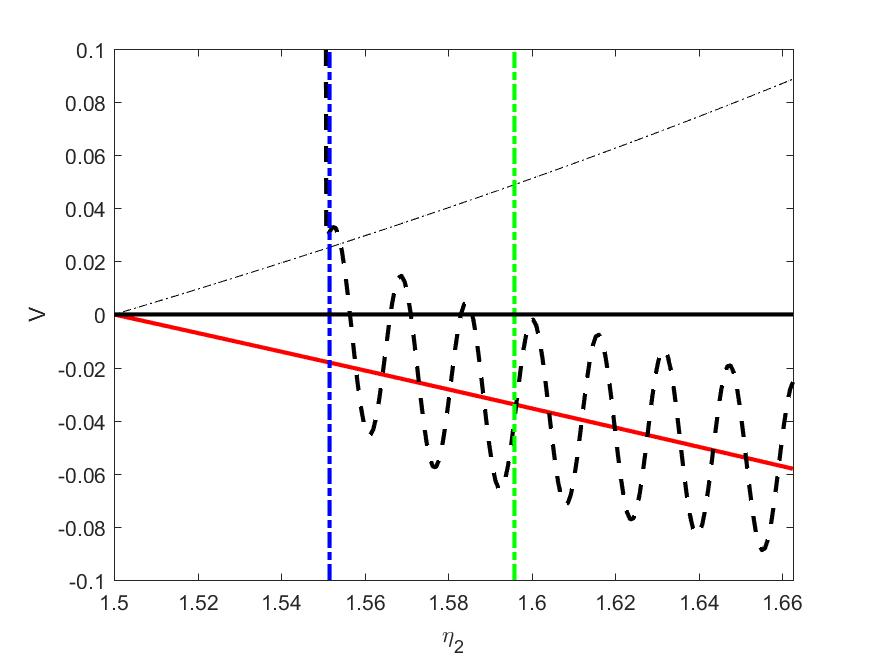
\includegraphics[scale=.25]{twoD/osc_cases.jpg}
\caption{Here we have the parameter ranges for Case I and Case II shown as the right most green vertical line and the bifurcation at the left blue vertical line respectfully.}
\label{fig:twoD_osc_cases}
\end{figure}

\subsection{Case I: $P_0(t)\le -|A|$}
\label{subsec:twoD_highfreqosc_caseI}

We call this the entirely below axis case, with the solution $X_0$ below the axis $V=0$ so that there is no bifurcation. This case helps to simplify the integration in \eqref{eq:twoD_osc_innerintegral} but also helps us to determine when the solution acts differently. Here we use the equilibria of $X$ and $Y$ to define a boundary between Case I and Case II. Under the conditions of this case, the system \eqref{eq:twoD_osc_innerintegral} simplifies to

\begin{equation}\label{eq:twoD_osc_caseIsystem}
\begin{aligned}
{P_0}_t(t) =& -n -\eta_3P_0(t)-(1-\eta_3)Q_0(t),\\
{Q_0}_t(t) =& \eta_1P_0(t)-Q_0(t).
\end{aligned}
\end{equation}

Solving for the equilibria in \eqref{eq:twoD_osc_caseIsystem} results in

\begin{equation*}
Q_0(P_0)=\eta_1P_0,\quad P_0=-\frac{n}{\eta_1(1-\eta_3)+\eta_3}. 
\end{equation*}

Together with these equilibria and with the condition $P_0(t)\le -|A|$, we find the parameter range that distinguishes between Case I and Case II in terms of our inner parameter, which we then rewrite in original coordinates with

\begin{equation}\label{eq:twoD_osc_boundary}
\begin{aligned}
n\ge& (\eta_1(1-\eta_3)+\eta_3)|A|,\\
\eta_2\ge&\eta_1\eta_3+ \frac{(\eta_1(1-\eta_3)+\eta_3)|A|}{\Omega}.
\end{aligned}
\end{equation}

For values of $\eta_2$ below the values given in \eqref{eq:twoD_osc_boundary}, we see the oscillations crossing above the axis $V=0$ and hence use a separate case to deal with this behavior.

\subsection{Case II: $|P_0(t)|<|A|$}
\label{subsec:twoD_highfreqosc_caseII}

We call this the crossing case; here the solution oscillates about the axis $V=0$ while the center of the oscillations approach the axis. With this behavior, we expect a bifurcation to occur in this region and thus we find the equilibria for \eqref{eq:twoD_osc_innerintegral} that determines the location. While this problem is two-dimensional in nature, the integral in \eqref{eq:twoD_osc_innerintegral} is nearly identical to the integral \eqref{eq:oneD_osc_integral} in \autoref{sec:oneD_highfreqosc}. So we may use the ideas of that section here to get an approximate solution. Thus, under the assumptions of this case, we fix a value of $P_0$ and integrate \eqref{eq:twoD_osc_innerintegral} over the regions defined by

\begin{equation*}
R_1=\arccos(P_0/A),\quad R_2=2\pi-\arccos(P_0/A).
\end{equation*}

As in \autoref{sec:oneD_highfreqosc}, the solution to \eqref{eq:twoD_osc_innerintegral} is negative for $P_0(t)$ the region $R\in[0,R_1]$ and alternates sign for the regions $R\in (R_1,R_2]$ and $R\in (R_2,2\pi]$. We follow the same procedure of integrating over each region to get the exact form for \eqref{eq:twoD_osc_innerintegral} with

\begin{equation}\label{eq:twoD_osc_caseIIexact}
\begin{aligned}
{P_0}_t=&-n- \eta_3 P_0(t)-(1-\eta_3)Q_0,\\
{Q_0}_t=&-\frac{2\eta_1}{\pi}\left(\arcsin(P_0/A)P_0+\sqrt{A^2-P_0^2}\right)-Q_0.
\end{aligned}
\end{equation}

Although this is the explicit inner equation from \eqref{eq:twoD_osc_caseIIexact}, this is analytically too complex to find an explicit form for a bifurcation and thus we use a second order Taylor approximation to give an approximate system

\begin{equation}\label{eq:twoD_osc_taylor}
\begin{aligned}
{P_0}_t=&-n -\eta_3 P_0-(1-\eta_3)Q_0,\\
{Q_0}_t=&-\frac{2\eta_1|A|}{\pi}-Q_0-\frac{\eta_1}{\pi|A|}P_0^2.
\end{aligned}
\end{equation}

We solve for the equilibria of \eqref{eq:twoD_osc_taylor} in order to locate the bifurcation. For simplicity, we define $a=\frac{\eta_1}{\pi|A|}$, and $ c=\frac{2\eta_1|A|}{\pi}$, then the equilibria satisfy

\begin{equation}\label{eq:twoD_osc_equilibria}
\begin{aligned}
Q_0(P_0)=&-aP_0^2-c,\\
0=-n+(1-\eta_3)c&-\eta_3 P_0+aP_0^2.
\end{aligned}
\end{equation}

Here the equation for $P_0$ in \eqref{eq:twoD_osc_equilibria} is a quadratic that would have two solutions, with the situation of following the lower branch given by negative solution with

\begin{equation}\label{eq:twoD_osc_innersolution}
P_0=\frac{\eta_3}{2a(1-\eta_3)}- \frac{1}{2a(1-\eta_3)}\sqrt{\eta_3^2+4a(1-\eta_3)(n-c(1-\eta_3))}.
\end{equation}

The equilibrium for $P_0$ in \eqref{eq:twoD_osc_innersolution} are real only for positive discriminant. Then the inner bifurcation, $n_{\text{osc}}$, is given for vanishing discriminant 

\begin{equation}\label{eq:twoD_osc_innerbif}
n_{osc} = \frac{\eta_1(1-\eta_3)|A|}{\pi}\left[2-\left(\frac{\pi\eta_3}{2\eta_1(1-\eta_3)}\right)^2\right].
\end{equation}

Here the equilibria in \eqref{eq:twoD_osc_equilibria} are given in terms of the inner variables. We write the solution for $V$, $T$ and bifurcation, ${\eta_2}_{\text{osc}}$, in the original coordinates

\begin{equation}\label{eq:twoD_osc_innersolnoriginal}
\begin{aligned}
V(t)\sim& \Omega^{-1}\left(P_0-A\cos(\Omega t)\right),\\
T(t)\sim& \eta_1-\Omega^{-1}\left(\frac{\eta_1}{\pi|A|}P_0^2+\frac{2\eta_1|A|}{\pi}+B\cos(\Omega t)\right),
\end{aligned}
\end{equation}

\begin{equation}\label{eq:twoD_osc_bifurcation}
{\eta_2}_{osc} = \eta_1\eta_3+\frac{\eta_1(1-\eta_3)|A|}{\pi\Omega}\left[2-\left(\frac{\pi\eta_3}{2\eta_1(1-\eta_3)}\right)^2\right].
\end{equation}

With \eqref{eq:twoD_osc_bifurcation} we have found the bifurcation induced by the addition of oscillatory forcing in the Stommel model. As we learned from the one-dimensional model in \autoref{sec:oneD_highfreqosc}, the effect of oscillatory forcing is bifurcations where ${\eta_2}_{\text{osc}}>{\eta_2}_{\text{ns}}$. Our result in \eqref{eq:twoD_osc_bifurcation} under the caveat that we restrict the parameters with 

\begin{equation*}
\eta_3 <\frac{2\sqrt{2}\eta_1}{\pi+2\sqrt{2}\eta_1},
\end{equation*}

which is the condition to guarantee the second term in \eqref{eq:twoD_osc_bifurcation} is positive. This restriction is reasonable as generally the parameters have the behaviors of $\eta_3<1$ and $\eta_3\ll \eta_1$ where the thermal variation is much larger in real ocean dynamics than the ratio of relaxation times.

In figure~\ref{fig:twoD_osc_Vnumerics} the numerical solution to \eqref{eq:twoD_canonical} for $V$ and a zoom of the solution around the numerical bifurcation is shown. The static bifurcation diagram is underlayed as well for comparison. We contrast the result in \eqref{eq:twoD_osc_bifurcation} to these numerics and find the bifurcation prediction from our analysis agrees. Notice that there is a bifurcation for $\eta_2>{eta_2}_{\text{ns}}$ with the oscillations present. This causes a region of the static lower branch in $V$ to never be followed.
In figure~\ref{fig:twoD_osc_Tnumerics} the numerical solution to \eqref{eq:twoD_canonical} for $T$ and a zoom in around the bifurcation is shown. Once more, the static bifurcation diagram is underlayed and we have two interesting features to note. Due to the bifurcation in $V$ for $\eta_2>{\eta_2}_{\text{ns}}$, the maximum value of $T$ is never reached in (b).

\begin{figure}[H]
\centering
\begin{subfigure}{.5\textwidth}
  \centering
  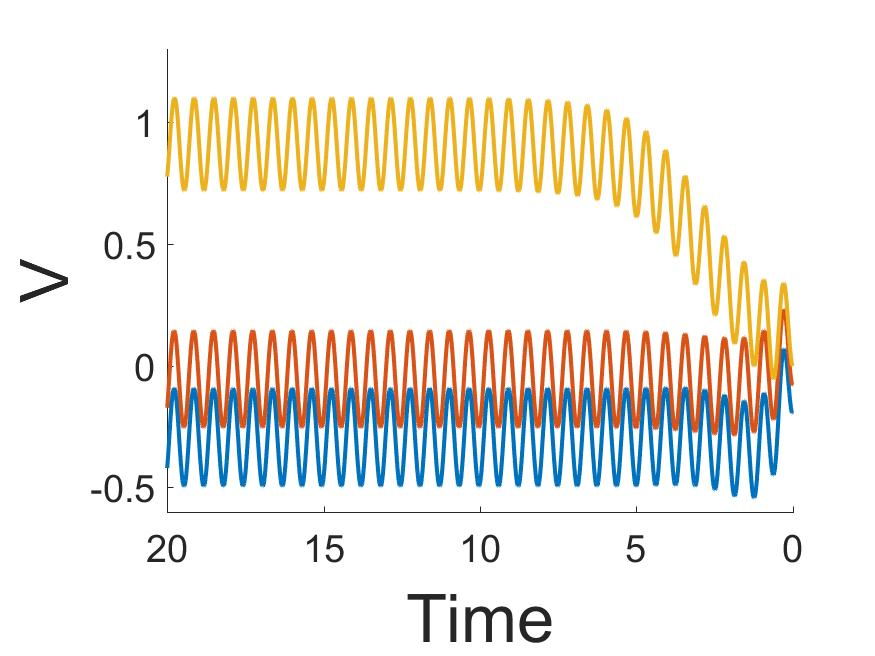
\includegraphics[width=\linewidth]{twoD/osc_Vtimeseries.jpg}
  \caption{}
\end{subfigure}%
\begin{subfigure}{.5\textwidth}
  \centering
  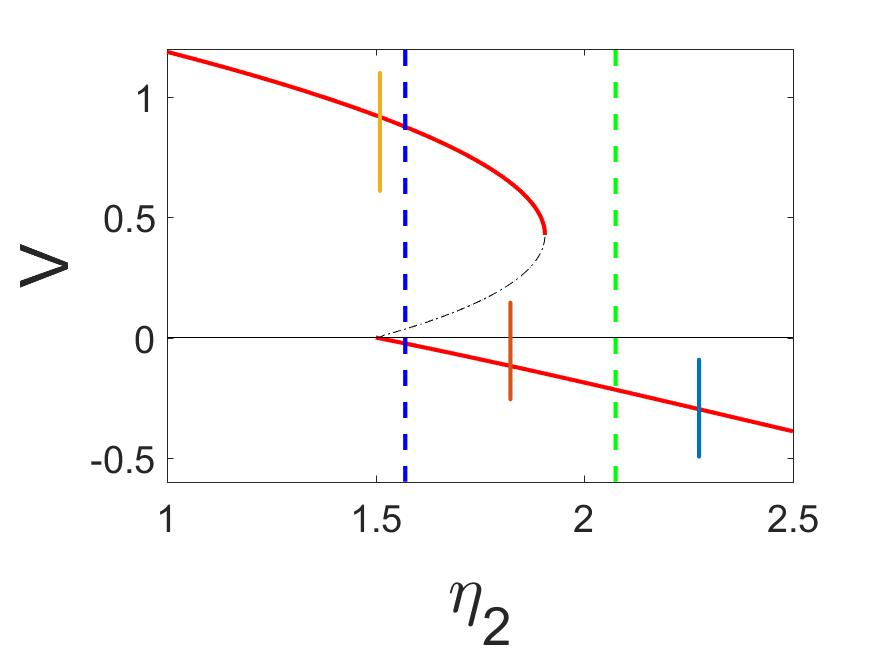
\includegraphics[width=\linewidth]{twoD/osc_bif_diagram.jpg}
  \caption{}
\end{subfigure}
\begin{subfigure}{.5\textwidth}
  \centering
  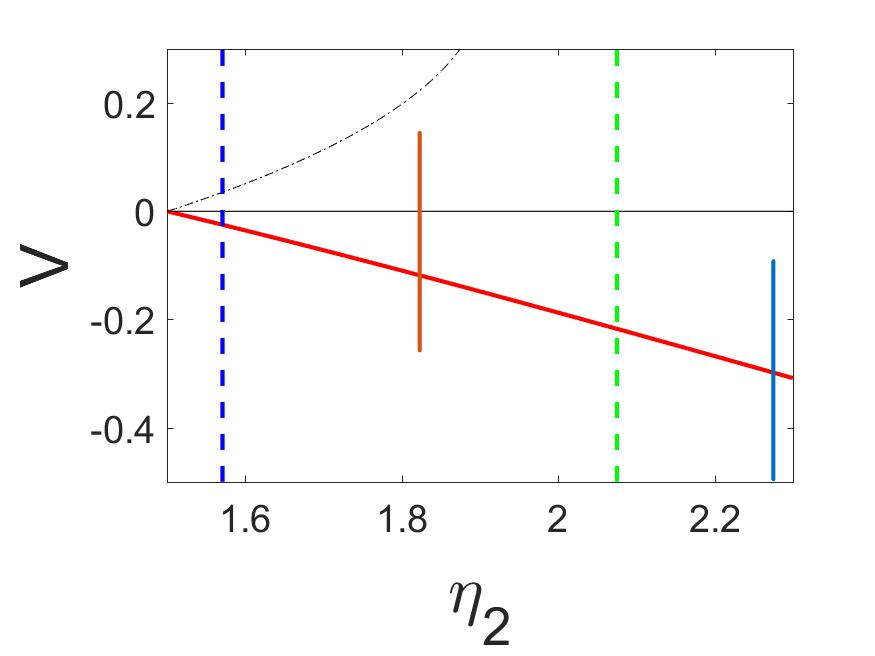
\includegraphics[width=\linewidth]{twoD/osc_bif_diagram_zoom.jpg}
  \caption{}
\end{subfigure}
\caption{In (a) the numerical time series solutions to \eqref{eq:twoD_canonical} is given with parameters in each qualitatively different case of $\eta_2=\{2.3,1.8,1.51\}$ with $\eta_1=4$, $\eta_3=.375$, $A=10$ and $\Omega = 10$. In (b) these same solutions are shown on the bifurcation diagram. In (c) a zoom in closer to the non-smooth bifurcation region where the blue vertical line is the prediction \eqref{eq:twoD_osc_bifurcation} against the black dotted vertical line which is the numerical bifurcation.}
\label{fig:twoD_osc_Vnumerics}
\end{figure}

\begin{figure}[H]
\centering
\begin{subfigure}{.5\textwidth}
  \centering
  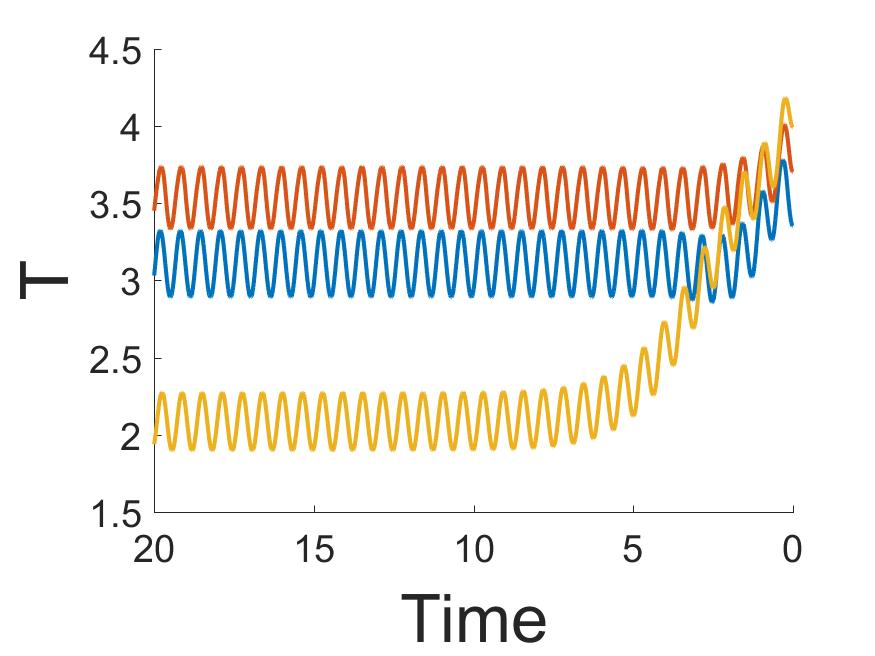
\includegraphics[width=\linewidth]{twoD/osc_Ttimeseries.jpg}
  \caption{}
\end{subfigure}%
\begin{subfigure}{.5\textwidth}
  \centering
  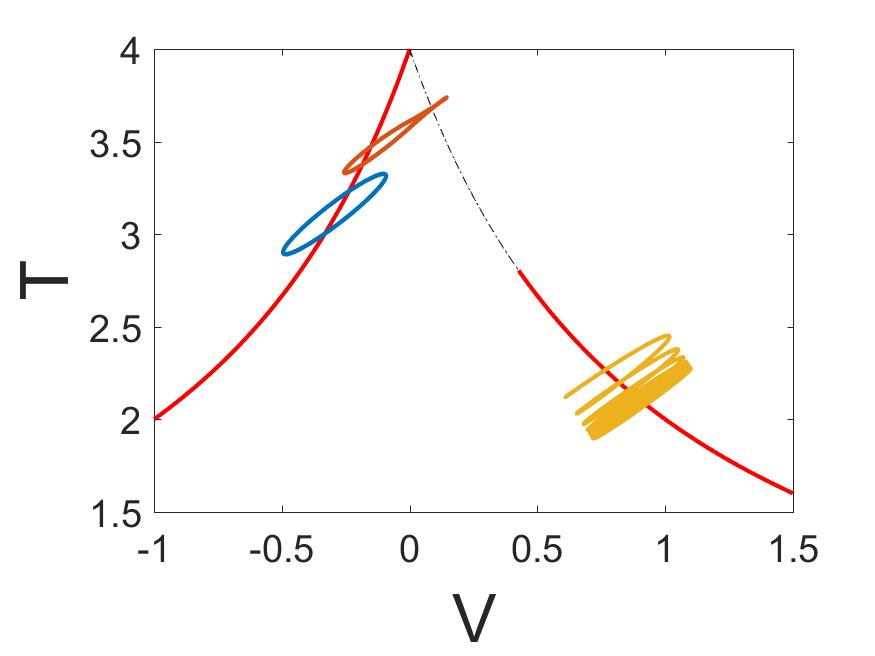
\includegraphics[width=\linewidth]{twoD/osc_bif_Tplot.jpg}
  \caption{}
\end{subfigure}
\begin{subfigure}{.5\textwidth}
  \centering
  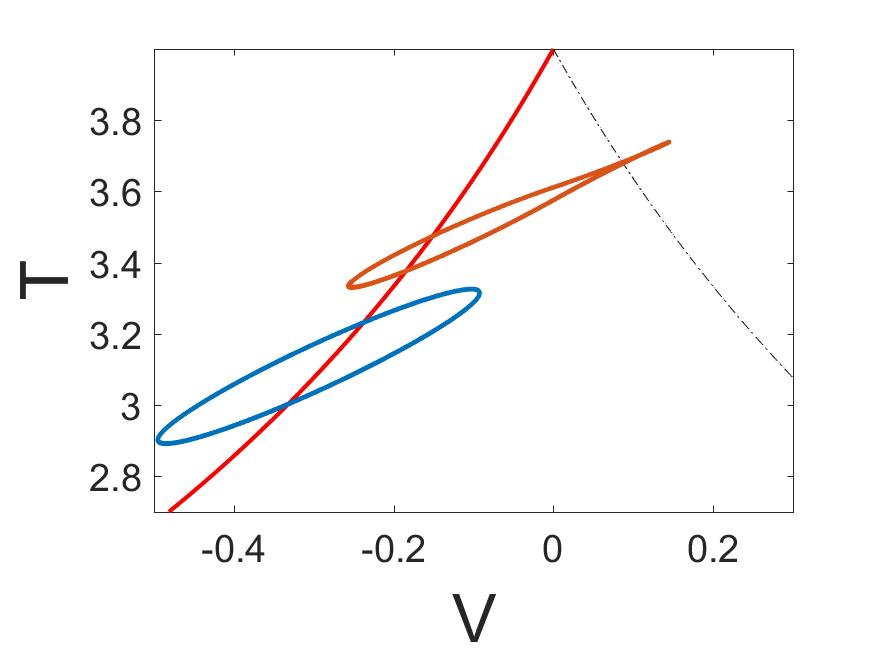
\includegraphics[width=\linewidth]{twoD/osc_bif_Tplot_zoom.jpg}
  \caption{}
\end{subfigure}
\caption{In (a) we have the numerical time series solutions for a qualitatively different cases $\eta_2=\{2.3,1.8,1.51\}$. In (b) we plot these solutions over the standard equilibrium plot for $V$ vs. $T$. In (c) a zoom of the bifurcation area.}
\label{fig:twoD_osc_Tnumerics}
\end{figure}

To evaluate the performance of this prediction, we compare \eqref{eq:twoD_osc_bifurcation} to the numerical bifurcation over a range of $\Omega^{-1}$. In figure~\ref{fig:twoD_osc_epscomp} we allow for this range to be $\Omega^{-1}\in (0,.5)$. For small values, the two agree very well and as we expect, they begin to diverge once the values of $\Omega^{-1}$ become too large from the assumption that $\Omega\gg 1$ and the asymptotics cannot capture the behavior for low frequency oscillations. But under our assumptions, the prediction is performing quite well and resembles the performance of \autoref{sec:oneD_highfreqosc}.

\begin{figure}[H]
\centering
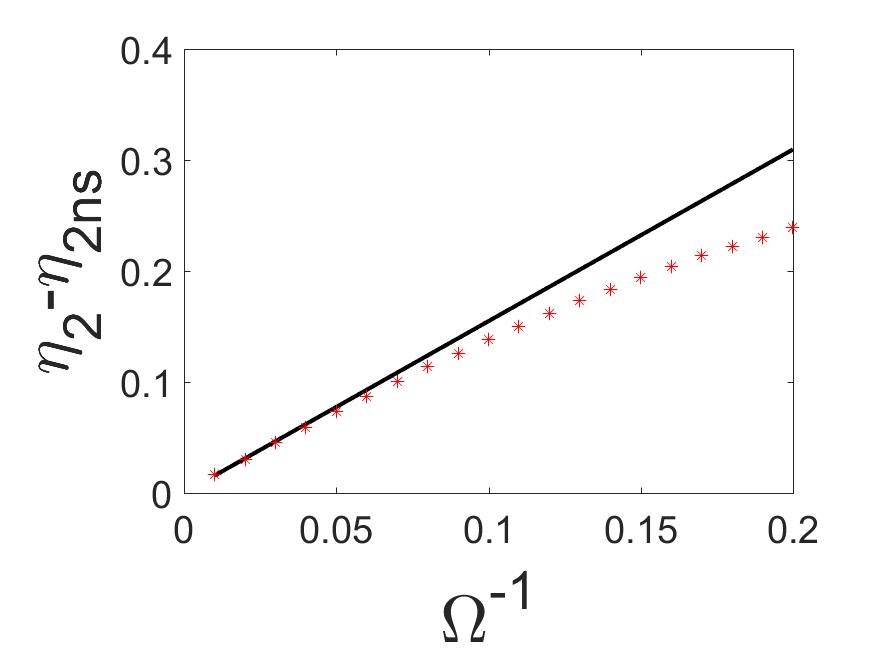
\includegraphics[scale=.25]{twoD/osc_Omegacomp.jpg}
\caption{The numerical tipping vs the estimate with $\eta_1=4$ and $\eta_3=\frac{3}{8}$. The bifurcation is when $V>.5$.}
\label{fig:twoD_osc_epscomp}
\end{figure}

\subsection{Stability}

Since we have a non-autonomous system when $A\not=0$, we approach the stability with a linearized analysis about the equilibria much like in \autoref{sec:oneD_highfreqosc}. To do this, recall from \eqref{eq:twoD_osc_innerintegral} that we found the system

\begin{equation}\label{eq:twoD_osc_stabilityequation}
\begin{aligned}
{P_0}_t =& -n -\eta_3 P_0-(1-\eta_3)Q_0,\\
{Q_0}_t =& -\frac{\eta_1}{2\pi}\int_0^{2\pi}|P_0-A\cos(R)|\, dR - Q_0.
\end{aligned}
\end{equation}

We must consider the stability of solutions over the relative sizes of $P_0(t)$ with Case I: $P_0(t)\le -|A|$ and Case II: $|P_0(t)|\le |A|$.

\subsubsection{Case I: $v_0(t)\le -|A|$}

For this case the entirely below-axis case where the solution spends most of its time away from the axis $V=0$. We expected attraction around the lower branch and thus we expect stability here. Under these conditions, the inner equation \eqref{eq:twoD_osc_stabilityequation} simplifies to the equations

\begin{equation}\label{eq:twoD_osc_stability_caseI_fullinner}
\begin{aligned}
{P_0}_t =& -m -\eta_3 P_0-(1-\eta_3)Q_0,\\
{Q_0}_t =& \eta_1 P_0 - Q_0.
\end{aligned}
\end{equation}

The equilibria of \eqref{eq:twoD_osc_stability_caseI_fullinner} is found with $Q_0(P_0)=\eta_1 P_0$, and thus we find the following one-dimensional equation and equilibrium

\begin{equation}\label{eq:twoD_osc_stability_caseI_red}
{P_0}_t = -n -(\eta_3 +(1-\eta_3))Q_0=f(P_0),\quad Z^0 = -\frac{n}{\eta_3+\eta_1(1-\eta_3)}.
\end{equation}

Now we consider a simple linear perturbation about this equilibrium with $P_0(t)= Z^0+U(t)$ where $\lVert U(t) \rVert \ll 1$. Our standard Taylor expansion about the equilibrium $Z^0$ results in

\begin{equation}\label{eq:twoD_osc_stability_caseI_perteq}
\begin{aligned}
f(P_0)=&f(Z^0)+f_{P_0}(Z^0)(P_0-Z^0)+O((P_0-Z^0)^2),\\
U_t =& -(\eta_3+\eta_1(1-\eta_3))U
\end{aligned}
\end{equation}

From \eqref{eq:twoD_osc_stability_caseI_perteq} we now conclude the equilibrium $Z^0$ is hyperbolic and asymptotically stable due to the exponential decay in perturbations. Thus we find that no bifurcation occurs for this case which agrees with our findings for this case in the analysis for $\eta_2$ in \eqref{eq:twoD_osc_boundary}

\begin{equation*}
\eta_2 \ge \eta_1\eta_3 +\frac{(\eta_3+\eta_1(1-\eta_3))|A|}{\Omega}.
\end{equation*}


\subsubsection{Case II: $|P_0(t)|<|A|$}

We called this case the crossing case and here the solution experiences the non-smooth behavior when it crosses $V=0$. We expect the stability to fail under these conditions and we discovered in the analysis that the crossing $V=0$ gives \eqref{eq:twoD_osc_stabilityequation} in the form

\begin{equation}\label{eq:twoD_osc_stability_caseII_full}
\begin{aligned}
{P_0}_t =& -n-\eta_3 P_0-(1-\eta_3)Q_0,\\
{Q_0}_t =& -\frac{2\eta_1|A|}{\pi}-\frac{\eta_1}{\pi |A|}P_0^2-Q_0.
\end{aligned}
\end{equation}

As we search for the equilibria of \eqref{eq:twoD_osc_stability_caseII_full}, we find the equilibrium for $Q_0$ in terms of $P_0$  

\begin{equation*}
Q_0(P_0)=-\frac{2\eta_1|A|}{\pi}-\frac{\eta_1}{\pi |A|}P_0^2
\end{equation*}

which then gives the following inner equation with the chosen equilibrium for $P_0<0$

\begin{equation}\label{eq:twoD_osc_stability_caseII_inner}
\begin{aligned}
{P_0}_t=&-n+\frac{2\eta_1(|A|}{\pi}-\eta_3 P_0+\frac{\eta_1}{\pi |A|}P_0^2=f(P_0),\\
Z^0=&\frac{\pi |A|}{2\eta_1(1-\eta_3)}\left(\eta_3-\sqrt{\frac{4\eta_1(1-\eta_3)}{\pi|A|}(n-n_{\text{osc}})}\right).
\end{aligned}
\end{equation}

For simplicity we write $Z^0$ in terms of the inner bifurcation $n_{text{osc}}$ we found in the analysis with \eqref{eq:twoD_osc_innerbif}. We now consider a simple linear perturbation about this equilibrium in \eqref{eq:twoD_osc_stability_caseII_inner} with $P_0(t)=Z^0+U(t)$ where $\lVert U(t)\rVert\ll 1$. The standard Taylor expansion about the equilibrium is thus

\begin{equation}\label{eqLtwoD_osc_stability_caseII_perturb}
\begin{aligned}
f(P_0)=&f(Z^0)+f_{P_0}(Z^0)(P_0-Z^0)+O((P_0-Z^0)^2),\\
U_t=&- 2\sqrt{\frac{\eta_1(1-\eta_3)}{\pi|A|}(n-n_{\text{osc}})}U.
\end{aligned}
\end{equation}

Thus with \eqref{eqLtwoD_osc_stability_caseII_perturb} we learn that the perturbations $U(t)$ decay exponentially as long as the square-root is non-zero and we restrict our attention to real solutions so that our perturbations are real. Thus we have that $Z^0$ is a hyperbolic and asymptotically stable equilibrium for $P_0$ and thus we find stability in $Q_0$ as well. This gives stability for this region but we lose this stability once the square-root becomes zero, here when

\begin{equation*}
n_{osc} = \frac{\eta_1(1-\eta_3)|A|}{\pi}\left[2-\left(\frac{\pi\eta_3}{2\eta_1(1-\eta_3)}\right)^2\right].
\end{equation*}

This says the equilibrium $Z^0$ at this point is non-hyperbolic which is indicative of a bifurcation. This is in agreement with our analysis and thus we can say that the value found in \eqref{eq:twoD_osc_bifurcation} is the bifurcation under the oscillatory forcing.


\section{Slow Variation with Oscillatory Forcing}
\label{sec:twoD_slowosc}

With the one-dimensional model solved and both the slowly varying and high oscillatory two-dimensional components analyzed, we have all of the tools needed to analyze the full system \eqref{eq:twoD_canonical} with both $\epsilon \ll 1$ and $A,B\sim O(1)$ simultaneously. This is the most general setting we discuss in this thesis where we account for both a slowly varying $\eta_2$ that leads to abrupt changes seen in \cite{alley2003abrupt,marotzke2000abrupt,rahmstorf2000thermohaline} as well as oscillatory forcing in both equations in \eqref{eq:twoD_canonical} seen in \cite{roberts2017relaxation,huybers2005obliquity}. We search for the interaction of these mechanisms in the physical Stommel model. Under the framework of slowly varying parameters we expect to find tipping instead of a bifurcation and hence our method for finding the tipping point follows a mixture of both \autoref{sec:twoD_slow} and \autoref{sec:twoD_highfreqosc}. This procedure dictates that we search for inner behavior about the non-smooth bifurcation and to do so we need to solve the inner equation and estimate when this solution abruptly transitions towards the upper branch. Ultimately, we provide a solution that captures the abrupt change from the lower stable branch to the upper branch in the full Stommel model.

To begin, we take our standard approach of following the lower branch towards the non-smooth behavior with $V<0$ in \eqref{eq:twoD_canonical} which gives the following system  

\begin{equation}\label{eq:twoD_slowosc_outereqs}
 \begin{aligned}
   \dot{V} & =  \eta_1-\eta_2-T+\eta_3(T-V)+V^2+A\sin(\Omega t), \\
   \dot{T} & =  \eta_1-T(1-V)+B\sin(\Omega t),  \\
  \dot{\eta_2}  & =  -\epsilon.
  \end{aligned}
\end{equation}

As in \autoref{sec:oneD_slowosc}, we write the frequency in terms of the slow variation, $\Omega = \epsilon^{-\lambda}$ with exponent $\lambda>0$. This assumption allows us to find the irelative influence of the slowly varying parameter and fast oscillations on the tipping. We notice in \eqref{eq:twoD_slowosc_outereqs} that there is variation on a slow scale in $\eta_2(t)$ and on a fast scale in $\sin(\Omega t)$, so this suggests a multiple scales approach with 'slow' time $\tau = \epsilon t$ and 'fast' time $R=\epsilon^{-\lambda}t$. Using this approach in \eqref{eq:twoD_slowosc_outereqs} yields

\begin{equation}\label{eq:twoD_slowosc_multiouter}
 \begin{aligned}
V_R+\epsilon^{\lambda+1}V_\tau & = \epsilon^{\lambda} \left(\eta_1-\eta_2-		T+\eta_3(T-V)+V^2+A\sin(R)\right), \\
T_R+\epsilon^{\lambda+1}T_\tau & = \epsilon^{\lambda}\left( \eta_1-T(1-		  V)+B\sin(R)\right),  \\
	{\eta_2}_\tau  & =  -1.
\end{aligned}
\end{equation}
  
To approach the solution to the outer equations in \eqref{eq:twoD_slowosc_multiouter}, we use an asymptotic expansion using both $\epsilon^\lambda$ and integer powers as we have not specified the range of $\lambda$ and both could be significant. Thus our expansion is

\begin{equation}\label{eq:twoD_slowosc_outerexpansion}
	\begin{aligned}
		V(\tau,R)\sim& V_0(\tau,R)+\epsilon^\lambda 	V_1(\tau,R)+O(\epsilon^{2\lambda},\epsilon^{\lambda+1}),\\
        T(\tau,R)\sim& T_0(\tau,R)+\epsilon^\lambda T_1(\tau,R)+O(\epsilon^{2\lambda},\epsilon^{\lambda+1}).
	\end{aligned}
\end{equation}

Here we substitute \eqref{eq:twoD_slowosc_outerexpansion} into \eqref{eq:twoD_slowosc_multiouter} to give

\begin{equation*}
\begin{aligned}
{V_0}_R+\epsilon^{\lambda+1}{V_0}_\tau+\epsilon^\lambda {V_1}_R+\ldots=&\begin{aligned}[t]&
\epsilon^\lambda \left(\eta_1-\eta_2-T+\eta_3(T_0-V_0)+V_0^2+A\sin(R)\right)\\
&+\epsilon^{2\lambda}\left(-\eta_3 V_1-(1-\eta_3)T_1+2V_0V_1\right)+\ldots
\end{aligned}\\
{T_0}_R+\epsilon^{\lambda+1}{T_0}_\tau+\epsilon^\lambda {T_1}_R+\ldots=&\begin{aligned}[t]&
\epsilon^\lambda\left( \eta_1-T_0(1-V_0)+B\sin(R)\right)\\
&+\epsilon^{2\lambda}\left(-T_1+T_0V_1+T_1V_0\right)+\ldots
\end{aligned}
\end{aligned}
\end{equation*}

Separating the equation at each order of $\epsilon$ then gives the following sets of equations

\begin{align}
\label{eq:twoD_slowosc_outerO1}
O(1):\quad & \begin{cases}
	{V_0}_R =&  0, \\
	{T_0}_R =&  0,\\
\end{cases}\\
\label{eq:twoD_slowosc_outerO2}
O(\epsilon^\lambda):\quad & \begin{cases}
	{V_1}_R = & \eta_1-\eta_2(\tau) +\eta_3(T_0-V_0)-T_0+V_0^2+A\sin(R),\\
	{T_1}_R =&  \eta_1-T_0(1-V_0)+B\sin(R),
\end{cases}\\
\label{eq:twoD_slowosc_outerO3}
O(\epsilon^{2\lambda}):\quad & \begin{cases}
	{V_2}_R+\epsilon^{1-\lambda}{V_0}_\tau = & \eta_3(T_1-V_1)-T_1+2V_0V_1,\\
	{T_2}_R +\epsilon^{1-\lambda}{T_0}_\tau =&  -T_1(1-V_0)+T_0V_1,
\end{cases}
\end{align}

Here we consider a $\lambda$ where the next order in \eqref{eq:twoD_slowosc_outerexpansion} is $O(\epsilon^{2\lambda})$. Similar results follow from a choice in $\lambda$ where $O(\epsilon^{\lambda+1})<O(\epsilon^{2\lambda})$. From \eqref{eq:twoD_slowosc_outerO1} the leading order terms in our expansion are only dependent on 'slow' time, $V_0=V_0(\tau)$ and $T_0=T_0(\tau)$. The solutions of \eqref{eq:twoD_slowosc_outerO2} and \eqref{eq:twoD_slowosc_outerO3} are found in \autoref{app:twoD}, giving the outer solution 

\begin{equation}\label{eq:twoD_slowosc_outersoln}
\begin{aligned}
V\sim& V_0 + \frac{\epsilon({V_0}_\tau(1-V_0)+(1-\eta_3){T_0}_\tau)}{(1-\eta_3)T_0+(2V_0-\eta_3)(1-V_0)}-\epsilon^\lambda A \cos(\Omega t),\\
T\sim& T_0 + \frac{\epsilon {T_0}_\tau}{1-V_0}-\frac{\epsilon T_0({V_0}_\tau(1-V_0)+(1-\eta_3){T_0}_\tau)}{(1-\eta_3)T_0(1-V_0)+(2V_0-\eta_3)(1-V_0)^2}-\epsilon^\lambda B \cos(\Omega t),
\end{aligned}
\end{equation}

where $V_0$ and $T_0$ are the same leading order solutions from the slowly varying Stommel model in \autoref{sec:twoD_slow}. Unfortunately the common theme of the Stommel model is that these outer solutions are complex but it is clear the outer expansion breaks down for $V_0\ll 1$. Thus we derive a scaling for the inner equations analogous to that of \autoref{sec:oneD_slowosc}.

For simplicity, we assume that the scaling for both $V$ and $T$ are the same, but this isn't necessary to arrive at the same conclusion. Hence we rescale about the bifurcation point $(V,T,\eta_2)=(0,\eta_1,\eta_1\eta_3)$ with

\begin{equation}\label{eq:twoD_slowosc_general_scaling}
V=\epsilon^\alpha X, \quad T=\eta_1+\epsilon^\alpha Y ,\quad \eta_2(t)=\eta_1\eta_3+\epsilon^\beta n(t),
\end{equation}

where both $\alpha>0$ and $\beta>0$ allow for this to be a local scaling. Applying the scalings in \eqref{eq:twoD_slowosc_general_scaling} to the full Stommel model \eqref{eq:twoD_canonical} gives

\begin{equation}\label{eq:twoD_slowosc_innerscaled}
\begin{aligned}
\epsilon^\alpha \dot{X}=& -\epsilon^\beta n(t)-\epsilon^\alpha (X+(1-\eta_3)Y) - \epsilon^{2\alpha}X|X| +A\sin(\epsilon^{-\lambda}t),\\
\epsilon^\alpha \dot{Y}=&-\epsilon^\alpha(\eta_1|X|+Y)+\epsilon^{2\alpha}|X|Y +B\sin(\epsilon^{-\lambda} t)\\
\dot{n}=&-\epsilon^{1-\beta}.
\end{aligned}
\end{equation}

From \eqref{eq:twoD_slowosc_innerscaled} it is apparent that there is still 'fast' behavior within the oscillations. Also note that due to the scaling in \eqref{eq:twoD_slowosc_general_scaling}, the local variables 'slow' behavior has been moved into the regular time $t$. To flesh out the particular choice in $\alpha$, we then take a multiple scales approach to capture the oscillations with $t$ and $R=\epsilon^{-\lambda}t$.  This choice comes with the ambiguity in $\beta$ and is discussed further below. Applying the multiple scales in \eqref{eq:twoD_slowosc_innerscaled} results in

\begin{equation}\label{eq:twoD_slowosc_innergeneral}
\begin{aligned}
\epsilon^{\alpha-\lambda} X_R+\epsilon^{\alpha}X_t=& -\epsilon^{\beta}n(t)-\epsilon^{\alpha}(X+(1-\eta_3)Y)-\epsilon^{2\alpha}X|X|+A\sin(R),\\
\epsilon^{\alpha-\lambda}Y_R + \epsilon^{\alpha}Y_t =&- \epsilon^\alpha(\eta_1|X|+Y)-\epsilon^{2\alpha}|X|Y +B\sin(R)\\
n_t=&-\epsilon^{1-\beta}.
\end{aligned}
\end{equation}

Here we balance the leading order terms in each equation of \eqref{eq:twoD_slowosc_innergeneral}, $\epsilon^{\alpha-\lambda}X_R$ and $A\sin(R)$ as well as $\epsilon^{\alpha-\lambda}Y_R$ with $B\sin(R)$, which gives us that $\alpha=\lambda$ and confirms that the scales $V$ and $T$ are the same. The scaling for $\eta_2$ has yet to be determined and could have multiple possibilities depending on $\lambda$, but due to this choice in $\alpha$ we expect the oscillatory term to persist in the inner asymptotic expansion of \eqref{eq:twoD_canonical} regardless of choice in $\lambda$.

We use a multiple scales approach with $t$ and $R=\epsilon^{-\lambda}t$ on the full Stommel model \eqref{eq:twoD_canonical} along with the general scaling \eqref{eq:twoD_slowosc_general_scaling} on $\eta_2$ which gives

\begin{equation}\label{eq:twoD_slowosc_general_outermulti}
\begin{aligned}
V_R+\epsilon^{\lambda}V_t =& -\epsilon^{\lambda+\beta}n(t)-\epsilon^{\lambda}(\eta_1-\eta_1\eta_3+\eta_3(T-V)-T-V|V|+A\sin(R)),\\
T_R+\epsilon^{\lambda}T_t =& \epsilon^\lambda(\eta_1-T(1+|V|)+B\sin(R)),\\
n_t =&-\epsilon^{1-\beta}.
\end{aligned}
\end{equation}

In \autoref{sec:oneD_slowosc} the results depended on the relative size of the slow variation with respect to the oscillations. The distinction in that case was when $\lambda\le1$ where a mixture between the slow variation and oscillations influence the tipping or $\lambda>1$ where the slow variation dominates the tipping. We find a similar distinction here and hence consider a separate asymptotic expansion for the following Case I: $\lambda\le 1$ and Case II: $\lambda >1$ to find an accurate classification of behavior for the full Stommel model.

\subsection{Case I: $\lambda \le 1$}

We call this the mixed effects case where there is significant influence from both slow variation and fast oscillations due to the size of $\lambda$. Here we cannot determine what the next term in the expansion should be and thus we choose a general expansion with

\begin{equation}\label{eq:twoD_slowosc_caseI_expansion}
\begin{aligned}
V(t,R)\sim& \epsilon^{\lambda} X_0(t,R)+\epsilon^q X_1(t,R)+\ldots\\
T(t,R)\sim& \eta_1+\epsilon^{\lambda} Y_0(t,R)+\epsilon^q Y_1(t,R)+\ldots
\end{aligned}
\end{equation}

with $q>\lambda$ to be consist with our analysis thus far. Substituting \eqref{eq:twoD_slowosc_caseI_expansion} into \eqref{eq:twoD_slowosc_general_outermulti} then gives the governing dynamics for this case

\begin{equation*}
\begin{aligned}
 {X_0}_R+\epsilon^{\lambda}{X_0}_t+\epsilon^{q-\lambda} {X_1}_R\ldots={} & -\epsilon^{\beta}n(t)-\epsilon^{\lambda} (\eta_3X_0+(1-\eta_3)Y_0) \\
&-\epsilon^{2\lambda}(X_0+\epsilon^{q-\lambda} X_1+\ldots)|X_0+\epsilon^{q-\lambda} X_1+\ldots|\\
& - \epsilon^{q}(\eta_3X_1+(1-\eta_3)Y_1) + A\sin(R) +\ldots
\end{aligned}
\end{equation*}

\begin{equation*}
\begin{aligned}
{Y_0}_R+\epsilon^{\lambda}{Y_0}_t+\epsilon^{q-\lambda} {Y_1}_R+\ldots= &-\epsilon^\lambda(\eta_1| X_0 +\epsilon^{q-\lambda} X_1+\ldots|+ Y_0+\epsilon^{q-\lambda} Y_1+\ldots)\\
&+\epsilon^{2\lambda}|X_0 +\epsilon^{q-\lambda} X_1+\ldots|(Y_0+\epsilon^{q-\lambda} Y_1+\ldots)\\
&+ B\sin (R)+\ldots
\end{aligned}
\end{equation*}

We separate by the distinct orders of $\epsilon$ to find the following equations at each order

\begin{align} \label{eq:twoD_slowosc_caseI_O1}
O(1):\, &\begin{cases}
	{X_0}_R =&  A\sin(R), \\
	{Y_0}_R =&  B\sin(R),\\
\end{cases}\\ \label{eq:twoD_slowosc_caseI_O2}
O(\epsilon^\lambda): \, & \begin{cases}
	\epsilon^{q-2\lambda}{X_1}_R+{X_0}_t =&  -\epsilon^{\beta-\lambda} n(t) -\eta_3 X_0-(1-\eta_3)X_0, \\
	\epsilon^{q-2\lambda}{Y_1}_R+{Y_0}_t =&  -\eta_1|X_0|-Y_0.\\
\end{cases}
\end{align}

We learn from \eqref{eq:twoD_slowosc_caseI_O2} that $q= 2\lambda$ balances the terms, which implies that $\lambda> \frac{1}{2}$ for an expansion to be found. If $\lambda\le \frac{1}{2}$ then we would need to include the quadratic terms in $O(\epsilon^\lambda)$ and our equations would just be the same as the full Stommel model \eqref{eq:twoD_canonical}. This indicated that our local approximation would no longer hold and that the high frequency assumption is failing. Without this, the physical behavior of the problem is qualitatively different and this we explore in the conclusion in \autoref{chap:conclusion}. On this range of $\lambda$, there are two choices for the scaling of $\eta_2$ with $\beta=1$ or $\beta=\lambda$. The advantage to choosing $\beta=\lambda$ is that the equation \eqref{eq:twoD_slowosc_caseI_O2} is simple, but the slow variation equation has the form $n_t = -\epsilon^{1-\lambda}$ and implies a slower time scale. On the other hand, $\beta=1$ keeps a small coefficient on $n$ in \eqref{eq:twoD_slowosc_caseI_O2} but gives the slow variation equation as $n_t=-1$, which allows the time scale $t$ to be used. Both of these choices result in the same approximation of the tipping point in original coordinates, so here we choose $\beta=1$ for convenience. From \eqref{eq:twoD_slowosc_caseI_O1} we find the appropriate form of the leading order terms, $X_0=P_0(t)-A\cos(R)$ and $Y_0=Q_0(t)-B\cos(R)$. Using these forms for the leading order term and applying the Fredholm alternative \eqref{eq:Fredholm} to \eqref{eq:twoD_slowosc_caseI_O2} we find 

\begin{equation}\label{eq:twoD_slowosc_caseI_fullinner}
\begin{aligned}
{P_0}_t =&  -\epsilon^{1-\lambda} n(t) -\eta_3 P_0-(1-\eta_3)Q_0, \\
{Q_0}_t =&  -\frac{\eta_1}{2\pi}\int_0^{2\pi}|P_0(t)-A\cos(R)|\,dR-Q_0,\\
n_t =& -1.
\end{aligned}
\end{equation}

We learned in \autoref{sec:twoD_highfreqosc} that we must approach the integration with the relative size of $P_0(t)$ to the amplitude of oscillation $A$ in mind as these sizes determine the contributions of the integral in \eqref{eq:twoD_slowosc_caseI_fullinner}. We consider these sizes of $P_0(t)$ as Sub-Case I: $P_0(t)\le -|A|$ and Sub-Case II:$|P_0(t)|<|A|$ similar to \autoref{sec:twoD_highfreqosc}. These cases let $P_0-A\cos(R)$ either stay entirely below $V=0$ or change signs respectively and allow the integration to have two distinct forms.

\subsubsection{Sub-Case I: $P_0(t)\le -|A|$}

We call this the below-axis sub-case where the solution $P_0(t)$ is entirely below the axis $V=0$ and this means the full solution $X_0$ has oscillations far from crossing. Under these conditions we don't expect any tipping behavior as the solution is far from $V=0$, but we may use this size of $P_0(t)$ to find the range of $\eta_2$ that distinguishes these cases. With $P_0(t)\le -|A|$, we find \eqref{eq:twoD_slowosc_caseI_fullinner} simplifies to

\begin{equation}\label{eq:twoD_slowosc_subcaseI_full}
\begin{aligned}
{P_0}_t =&  -\epsilon^{1-\lambda} n(t) -\eta_3 P_0-(1-\eta_3)Q_0, \\
{Q_0}_t =&  \eta_1 P_0-Q_0.
\end{aligned}
\end{equation}

We have the means available to solve \eqref{eq:twoD_slowosc_subcaseI_full} as it takes the form of an equation we have seen in \autoref{sec:twoD_slow}, but instead we search for when the pseudo-equilibrium fails the assumption of this sub-case. This results in the parameter range between these sub-cases and taking this approach is more convenient than solving the system. Here the form of the pseudo-equilibria is simple to find as $Q_0(P_0) = \eta_1P_0$ and thus 

\begin{equation*}
P_0(t) = -\epsilon^{1-\lambda}\frac{n(t)}{\eta_3+\eta_1(1-\eta_3)}.
\end{equation*}

But we recall that for this sub-case $P_0(t)\le -|A|$, which gives the range for $n$ and we rewrite this in the original coordinates of $\eta_2$ with

\begin{equation}\label{eq:twoD_slowosc_subcaseboundary}
\begin{aligned}
\epsilon n \ge & \epsilon^\lambda (\eta_3+\eta_1(1-\eta_3))|A|,\\
\eta_2 \ge& \eta_1\eta_3 +\frac{(\eta_3+\eta_1(1-\eta_3))|A|}{\Omega}.
\end{aligned}
\end{equation}

With the parameter range \eqref{eq:twoD_slowosc_subcaseboundary}, we now have an effective region for Sub-Case I and have the range for Sub-Case II in terms of the parameter $\eta_2$.

\subsubsection{Sub-Case II: $|P_0(t)|\le |A|$}

We call this the crossing sub-case and under these conditions we see the integral in \eqref{eq:twoD_slowosc_caseI_fullinner} is more complex. As this contribution changes, there is an increasing effect on the system and it is here that we anticipate the tipping to occur. In \autoref{sec:oneD_slowosc}, we found a similar integral to \eqref{eq:twoD_slowosc_caseI_fullinner} that we could evaluate with the assumption that $A\sim O(1)$. We find that the assumptions that allowed for evaluation of the integral in \eqref{eq:oneD_slowosc_caseIintegral} from \autoref{sec:oneD_slowosc} still hold here with a 'fast' time $R$ that is sufficiently large due to the high frequency. We then follow the approach from \autoref{sec:oneD_slowosc} by integrating with $R_1=\arccos(P_0/A)$ and $R_2 = 2\pi-\arccos(P_0/A)$ analogous to $T_1$ and $T_2$ from \autoref{sec:oneD_slowosc} Case I and then taking a quadratic Taylor approximation as in \eqref{eq:oneD_slowosc_subcaseIItaylor} gives

\begin{equation}\label{eq:twoD_slowosc_subcaseII_taylor}
\begin{aligned}
{P_0}_t =& -\epsilon^{1-\lambda}n(t)-\eta_3 P_0(s)-(1-\eta_3)Q_0\\
{Q_0}_t =&-\frac{2\eta_1|A|}{\pi}-\frac{\eta_1}{\pi|A|}P_0^2-Q_0.
\end{aligned}
\end{equation}

Here the form in \eqref{eq:twoD_slowosc_subcaseII_taylor} is known as a quadratic two-dimensional Riccati-type equation. We recall the assumption that the solution to the equation for $T$ to be in terms of $V$ was realistic to the THC, so any behavior that we are interested in lies within the dynamics for $V$, or it's inner counterpart $X$. For this reason, we choose to approximate by reducing \eqref{eq:twoD_slowosc_subcaseII_taylor} to a one-dimensional model by assuming our equation for $Q_0$ is in pseudo-equilibrium with 

\begin{equation}\label{eq:twoD_slowosc_subcaseII_equilreduction}
{Q_0}(P_0) =  -\frac{2\eta_1|A|}{\pi}-\frac{\eta_1}{\pi|A|}P_0^2.
\end{equation}

The resulting reduced system from introducing the equilibrium \eqref{eq:twoD_slowosc_subcaseII_equilreduction} into the leading order inner equation \eqref{eq:twoD_slowosc_subcaseII_taylor} is then

\begin{equation}\label{eq:twoD_slowosc_subcaseII_reducedeq}
\begin{aligned}
{P_0}_t =& -\epsilon^{1-\lambda}n(t)+\frac{2\eta_1(1-\eta_3)|A|}{\pi}-\eta_3P_0+\frac{\eta_1}{\pi|A|}P_0^2,\\
n_t=&-1.
\end{aligned}
\end{equation}

We rewrite the differentiation in \eqref{eq:twoD_slowosc_subcaseII_reducedeq} in terms of parameter $n$ giving 

\begin{equation} \label{eq:twoD_slowosc_subcaseII_reducedn}
\begin{aligned}
{P_0}_n =& \epsilon^{1-\lambda} n -\frac{2\eta_1(1-\eta_3)|A|}{\pi}+\eta_3 P_0-\frac{\eta_1(1-\eta_3)}{\pi|A|}P_0^2.\\
\end{aligned}
\end{equation}

Now \eqref{eq:twoD_slowosc_subcaseII_reducedn} is in a form when the result from Zhu \& Kuske \eqref{eq:intro_Zhueq} applies. Thus we determine that \eqref{eq:twoD_slowosc_subcaseII_reducedn} is an Airy-type equation and that the tipping point follows with \eqref{eq:intro_Zhuresult}. We write the solution in original coordinates and obtain results similar to previous sections with

\begin{equation}\label{eq:twoD_slowosc_subcaseII_tipping}
\begin{aligned}
n_{\text{tip}} =& -\epsilon^{(\lambda-1)/3}\left(\frac{\pi|A|}{\eta_1(1-\eta_3)}\right)^{1/3}(2.33810)+\epsilon^{\lambda-1}\frac{\eta_1(1-\eta_3)|A|}{\pi}\left(2-\left(\frac{\pi\eta_3}{2\eta_1(1-\eta_3)}\right)^2\right),\\
{\eta_2}_{\text{tip}} =& \epsilon^{(\lambda-1)/3}\left(\frac{\pi|A|}{\eta_1(1-\eta_3)}\right)^{1/3}\mu_{\text{smooth}}+{\eta_2}_{\text{osc}}
\end{aligned}
\end{equation}

We conclude that the tipping point in \eqref{eq:twoD_slowosc_subcaseII_tipping} has a similar fom as the tipping point found with \eqref{eq:oneD_slowosc_caseItipping} in \autoref{sec:oneD_slowosc} where we found a weighted average between the smooth tipping and the oscillatory bifurcation for this range of $\lambda$. We also found in \eqref{eq:twoD_slowosc_caseI_O2} that any choice for $\lambda\le\frac{1}{2}$ gave equations that can not be studied using the multiple scales approach in this section. This heuristically makes sense since for $\lambda\le \frac{1}{2}$ we have low frequency oscillations with our polynomial relationship and the contributions to the dynamics from this behavior require a different approach than presented in this paper. For more, see Zhu \& Kuske \cite{zhu2015tipping} for an example of a low-frequency method.

\subsection{Case II: $\lambda>1$}

We call this case the slow dominant case; here we expect integer powers of $\epsilon$ to appear due to the $O(\epsilon^\lambda)$ being quite small for this range of $\lambda$ and thus we choose the expansion 

\begin{equation}\label{eq:twoD_slowosc_caseII_expansion}
\begin{aligned}
V(t,R) \sim& \epsilon X_0(t,R)+\epsilon^\lambda X_1(t,R)+\epsilon^q X_2(t,R)+\ldots\\
T(t,R) \sim& \epsilon Y_0(s,R) + \epsilon^\lambda Y_1(t,R) +\epsilon^q Y_2(t,R)+\ldots
\end{aligned}
\end{equation}

Substituting \eqref{eq:twoD_slowosc_caseII_expansion} into \eqref{eq:twoD_slowosc_general_outermulti} then gives

\begin{equation*}
\begin{aligned}
\epsilon {X_0}_R+\epsilon^{\lambda+1}{X_0}_t+\epsilon^\lambda {X_1}_R+\ldots={} & -\epsilon^{\lambda+\beta}n(t)-\epsilon^{\lambda+1} (\eta_3X_0+(1-\eta_3)Y_0) \\
&-\epsilon^{\lambda+2}(X_0+\epsilon^{q-\lambda} X_1+\ldots)|X_0+\epsilon^{q-\lambda} X_1+\ldots|\\
& - \epsilon^{2\lambda}(\eta_3X_1+(1-\eta_3)Y_1) + \epsilon^\lambda A\sin(R),
\end{aligned}
\end{equation*}

\begin{equation*}
\begin{aligned}
\epsilon {Y_0}_R+\epsilon^{\lambda+1}{Y_0}_t+\epsilon^\lambda {Y_1}_R+\ldots=& -\epsilon^{\lambda+1}(\eta_1|X_0 +\epsilon^{\lambda-1} X_1+\epsilon^{q-1} X_2+\ldots|- Y_0-\epsilon^{\lambda-1} Y_1+\ldots)\\
&+\epsilon^2|X_0 +\epsilon^{\lambda-1} X_1+\epsilon^{q-1} X_2+\ldots|(Y_0 +\epsilon^{\lambda-1} Y_1+\ldots)\\
&+\epsilon^\lambda B \sin (R).
\end{aligned}
\end{equation*}

Here we separate by each distinct order of $\epsilon$ to find the following equations at each order of $\epsilon$

\begin{align} \label{eq:twoD_slowosc_caseII_O1}
O(\epsilon):\, &\begin{cases}
	{X_0}_R =& 0, \\
	{Y_0}_R =& 0,\\
\end{cases}\\ \label{eq:twoD_slowosc_caseII_O2}
O(\epsilon^\lambda): \, & \begin{cases}
	{X_1}_R =& A\sin(R), \\
	{Y_1}_R =& B\sin(R),\\
\end{cases}\\
\label{eq:twoD_slowosc_caseII_O3}
O(\epsilon^{\lambda+1}):\, &\begin{cases}
	\epsilon^{q-\lambda-1}{X_2}_R+{X_0}_t =& -\epsilon^{\beta-1}n(t)-\eta_3X_0-(1-\eta_3)Y_0, \\
	\epsilon^{q-\lambda-1}{Y_2}_R+{Y_0}_t =& -\eta_1|\epsilon^{\lambda}|X_0+\epsilon^{\lambda-1}X_1|-Y_0,\\
\end{cases}
\end{align}

We learn in \eqref{eq:twoD_slowosc_caseII_O3} that $q=\lambda+1$ balances terms in the expansion. We also find that $\beta =1$ gives both simple expressions in \eqref{eq:twoD_slowosc_caseII_O3} but also $n_t=-1$. Here a single choice is clear as opposed to Case I where we chose the value of $\beta$ for convenience. In \eqref{eq:twoD_slowosc_caseII_O1} we find that the leading order behavior for this case depends only on 'slow' time, $X_0=X_0(t)$ and $Y_0=Y_0(t)$, thus giving dominant behavior in this case. With \eqref{eq:twoD_slowosc_caseII_O2} we find the correction terms are given by $X_1=P_1(t)-A\cos(R)$ and $Y_1=Q_1(t)-B\cos(R)$ and since the slow behavior in $X_1$ and $Y_1$ are just next order corrections to the purely slow $X_0$ and $Y_0$, without loss of generality we set $P_1\equiv Q_1\equiv 0$; thus we have purely oscillatory corrections, $X_1=-A\cos(R)$ and $Y_1=-B\cos(R)$. Applying Fredholm \eqref{eq:Fredholm} to \eqref{eq:twoD_slowosc_caseII_O3} then gives

\begin{equation}\label{eq:twoD_slowosc_caseII_fullinner}
\begin{aligned}
{X_0}_t =& -n(t) -\eta_3 X_0- (1-\eta_3)Y_0,\\
{Y_0}_t =& -\frac{\eta_1}{2\pi}\int_0^{2\pi}|X_0(t)-\epsilon^{\lambda-1}A\cos(R)|\,dR -Y_0,\\
n_t=& -1.
\end{aligned}
\end{equation}

From Case I, we used the pseudo-equilibrium of $Q_0$ for an integral of this type regardless of the size of the oscillations to find a solvable equation. Here we expect \eqref{eq:twoD_slowosc_caseII_fullinner} to have some kind of quadratic form as Case I, so we choose a priori to use a similar reduction by assuming the equation for $Y_0$ is in it's pseudo-equilibrium with

\begin{equation}\label{eq:twoD_slowosc_caseII_equilreduction}
{Y_0}(X_0)= -\frac{\eta_1}{2\pi}\int_0^{2\pi}|X_0-\epsilon^{\lambda-1}A\cos(R)|\,dR.
\end{equation}

We find the resulting reduced one-dimensional equation by introducing \eqref{eq:twoD_slowosc_caseII_equilreduction} into the inner equation \eqref{eq:twoD_slowosc_caseII_fullinner} with

\begin{equation}\label{eq:twoD_slowosc_caseII_reducedeq}
{X_0}_t = -n(t)-\eta_3 X_0+\frac{\eta_1(1-\eta_3)}{2\pi}\int_0^{2\pi}|X_0(t)-\epsilon^{\lambda-1}A\cos(R)|\,dR.
\end{equation}

Here with \eqref{eq:twoD_slowosc_caseII_reducedeq} the behavior is very similar to Case I as long as the amplitude of oscillations inside the integral are consistent with the assumptions from that case, $\epsilon^{\lambda-1}A \sim O(1)$. With this assumption we have that $\lambda \approx 1$ to see mixed behavior of Case I and thus we once more follow the method of \autoref{sec:oneD_slowosc}. Our assumption on the size of the oscillations allow us to integrate \eqref{eq:twoD_slowosc_caseII_reducedeq} with $R_1= \arccos(x_0/\epsilon^{\lambda-1}A)$ and $R_2 = 2\pi - \arccos(x_0/\epsilon^{\lambda-1}A)$ analogous to $T_1$ and $T_2$ from \autoref{sec:oneD_slowosc} Case II. Another application of a quadratic Taylor approximation as in \eqref{eq:oneD_slowosc_caseII_taylor} then yields

\begin{equation}\label{eq:twoD_slowosc_caseII_taylor}
\begin{aligned}
{X_0}_t = -n(t) +\epsilon^{\lambda-1}\frac{2\eta_1(1-\eta_3)|A|}{\pi}-\eta_3 X_0 +\epsilon^{1-\lambda}\frac{\eta_1(1-\eta_3)}{\pi |A|}X_0^2.
\end{aligned}
\end{equation}

Once more, we find a form to which we apply the result from Zhu \& Kuske in \eqref{eq:intro_Zhueq} to. Thus we find the tipping point for the scaled parameter $n$ with \eqref{eq:intro_Zhuresult} and then transform back into the original coordinates for tipping in $\eta_2$ with

\begin{equation}
\begin{aligned}
n_{\text{mixed}}=&-\epsilon^{(\lambda-1)/3}\left(\frac{\pi|A|}{\eta_1(1-\eta_3)}\right)^{1/3}(2.33810)+\epsilon^{\lambda-1}\frac{\eta_1(1-\eta_3)|A|}{\pi}\left(2-\left(\frac{\pi\eta_3}{2\eta_1(1-\eta_3)}\right)^2\right),\\
{\eta_2}_{\text{mixed}}=& \epsilon^{(\lambda-1)/3}\left(\frac{\pi|A|}{\eta_1(1-\eta_3)}\right)^{1/3}\mu_{\text{smooth}}+{\eta_2}_{\text{osc}}.
\end{aligned}
\end{equation}

For $\lambda>1$ and away from 1, the amplitude of the oscillations is smaller, and inside the integral in \eqref{eq:twoD_slowosc_innergeneral} their contribution from the oscillations is reduced. Although no exact cut off exists and depending on the choice in other model parameters $\eta_1$ and $\eta_3$ we find that typically for $\lambda\ge 1.5$ the system \eqref{eq:twoD_slowosc_caseII_fullinner} is approximated by

\begin{equation}\label{eq:twoD_slowosc_caseII_sloweq}
\begin{aligned}
{X_0}_t =& -n(t)-\eta_3 X_0 -(1-\eta_3)Y_0,\\
{Y_0}_t =&-\eta_3|X_0|-Y_0,\\
n_t  =&-1.
\end{aligned}
\end{equation}

Here \eqref{eq:twoD_slowosc_caseII_sloweq} is the same system as the slowly varying model in \autoref{sec:twoD_slow}. With the same inner equation and slowly varying $n$, we are able to use the approximation found in \autoref{sec:twoD_slow} for the tipping point \eqref{eq:twoD_slow_tipping} here as well. This indicates that the amplitude of the oscillations are small for larger $\lambda$, so that only the slow variation affects the tipping of the Stommel model.

With both Case I and Case II, we have the tipping behavior for any choice in $\lambda$. For $\lambda\le1$, we found a similar combination of contributions from the oscillatory bifurcation and the smooth tipping in the Airy equation as in \autoref{sec:oneD_slowosc}. This behavior is observed for both $\lambda\le 1$ and $\lambda>1$ but the oscillatory behavior contributes less to the advance of the tipping point for larger $\lambda$. For $\lambda$ sufficiently large, the oscillations have a negligible contribution and we recover the tipping point for the purely slowly varying model. The results for the tipping point in the Stommel model with slowly varying parameter $\eta_2$ and oscillatory forcing is summarized in the following table.

\begin{table}[H]
\begin{center}
\begin{tabular}{|c|c|}
\hline 
 \multicolumn{2}{|c|}{Two-Dimensional Tipping} \\ 
\hline
$\epsilon>0$ and $A=0$ & ${\eta_2}_{\text{slow}}=\min(\eta_1\eta_3 -\epsilon\log(\epsilon)/\lambda_i)$ for $i\in\{1,2\}$ \\ 
\hline 
$\epsilon=0$ and $A\not=0$ with $\Omega\gg 1$ & ${\eta_2}_{\text{osc}}=\eta_1\eta_3+\frac{\eta_1(1-\eta_3)|A|}{\pi\Omega}\left(2-\left(\frac{\pi\eta_3}{2\eta_1(1-\eta_3)}\right)^2\right)$ \\ 
\hline 
$\epsilon>0$, $A\not=0$ and $\frac{1}{2}<\lambda\le 1$: & ${\eta_2}_{\text{mixed}}=\epsilon^{(\lambda-1)/3}\left(\frac{\pi |A|}{\eta_1(1-\eta_3)}\right)^{1/3} \mu_{\text{smooth}}+{\eta_2}_{\text{osc}}$ \\ 
\hline 
$\epsilon>0$, $A\not=0$ and $\lambda >1$ with $\lambda \approx 1$: &${\eta_2}_{\text{mixed}}=\epsilon^{(\lambda-1)/3}\left(\frac{\pi |A|}{\eta_1(1-\eta_3)}\right)^{1/3} \mu_{\text{smooth}}+{\eta_2}_{\text{osc}}$ \\ 
\hline 
$\epsilon>0$, $A\not=0$ and $\lambda>1$:
 & ${\eta_2}_{\text{slow}}=\min(\eta_1\eta_3 -\epsilon\log(\epsilon)/\lambda_i)$ for $i\in\{1,2\}$ \\
\hline
\end{tabular} 
\caption{The tipping of the two-dimensional model for each mechanism and case.}
\end{center}
\end{table}

In figure~\ref{fig:twoD_slowosc_Vnumerics_small}, we see an example of the numerical solution of $V$ to the Stommel model \eqref{eq:twoD_canonical} with slow variation and oscillatory forcing. This example illustrates tipping for Case I with $\lambda\in (\frac{1}{2},1]$, so that both the slow variation and oscillations influence tipping. The vertical lines are the tipping, black solid for the numerical and blue dotted for the approximation for this case \eqref{eq:twoD_slowosc_subcaseII_tipping}. Although there is a mixture of effects, the tipping gives a value near the oscillatory bifurcation. This tells us that for these choices in the model parameters that the strongest effect is the oscillatory forcing. The results are shown in figure \eqref{fig:twoD_slowosc_Tnumerics_small} in the $V-T$ plane. Here we see that due to the early tipping in $V$, the solution for $T$ also never achieves it's maximum and there is early tipping here as well, which agrees with the assumptions we had made of considering $T$ responding to $V$.

\begin{figure}[H]
\centering
\begin{subfigure}{.5\textwidth}
  \centering
  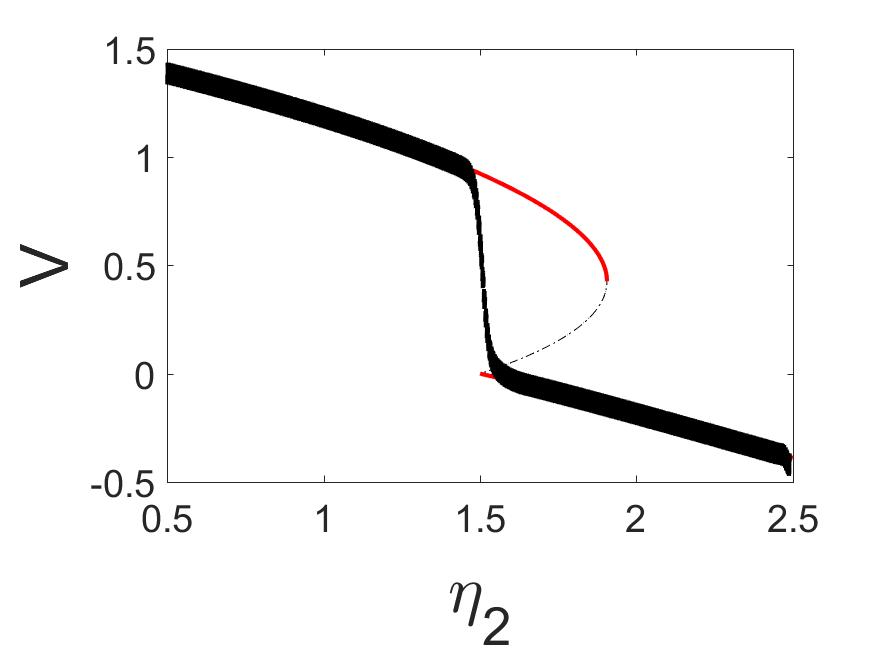
\includegraphics[width=\linewidth]{twoD/slowosc_bif_diagram_small.jpg}
  \caption{}
\end{subfigure}%
\begin{subfigure}{.5\textwidth}
  \centering
  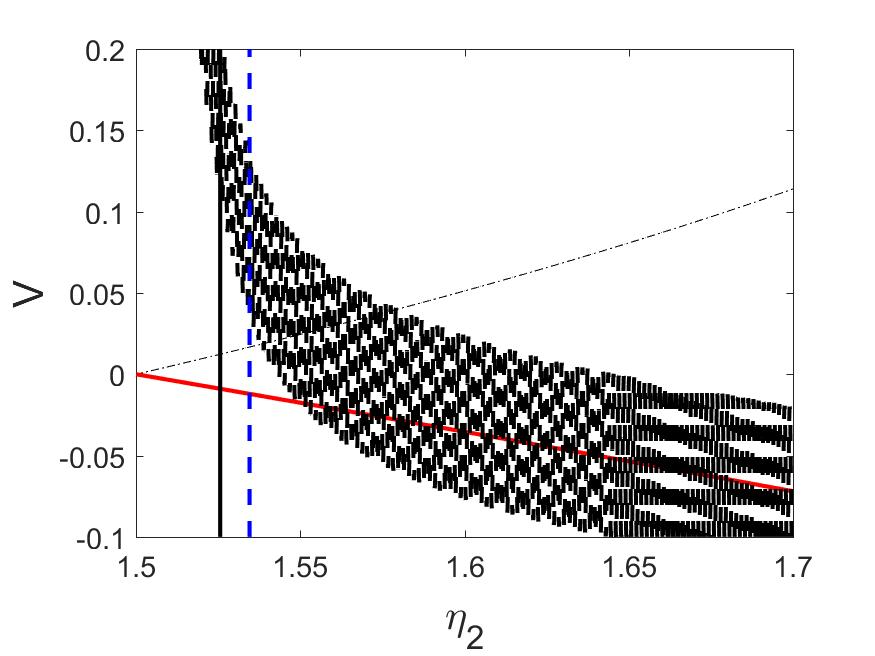
\includegraphics[width=\linewidth]{twoD/slowosc_bif_diagram_small_zoom.jpg}
  \caption{}
\end{subfigure}
\caption{Model values are $\lambda=.8$, $\epsilon=.01$ with $A=B=2$. In (a) the numerical solution (black dotted line) to \eqref{eq:twoD_canonical} is given with $\eta_1=4$, $\eta_3=.375$. In (b) a zoom in closer to the non-smooth bifurcation region where the blue dotted vertical line is the tipping point \eqref{eq:twoD_slowosc_subcaseII_tipping} and the black vertical line is the numerically obtained tipping for $V>V_{\text{smooth}}$.}
\label{fig:twoD_slowosc_Vnumerics_small}
\end{figure}

\begin{figure}[H]
\centering
\begin{subfigure}{.5\textwidth}
  \centering
  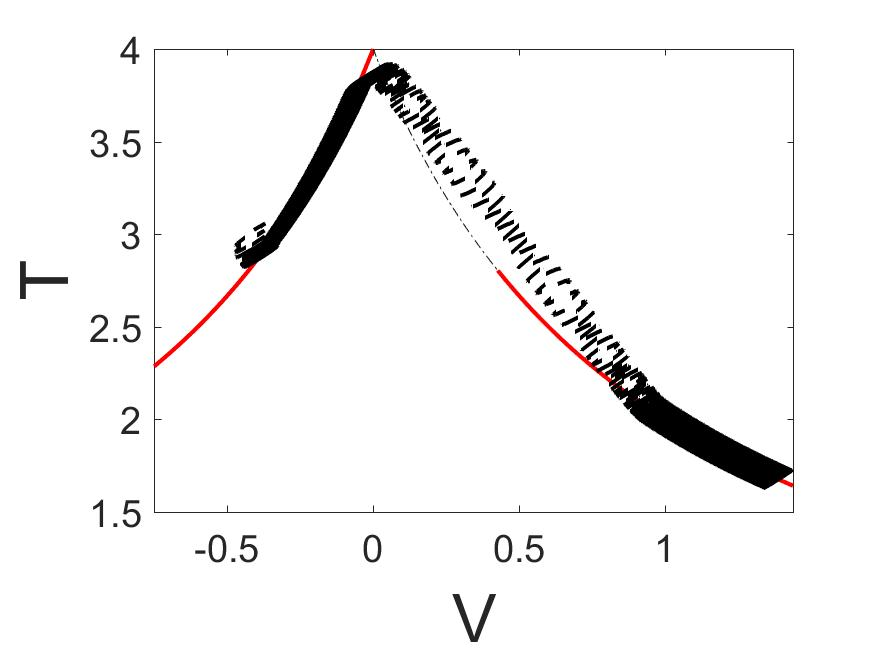
\includegraphics[width=\linewidth]{twoD/slowosc_Tplot_small.jpg}
  \caption{}
\end{subfigure}%
\begin{subfigure}{.5\textwidth}
  \centering
  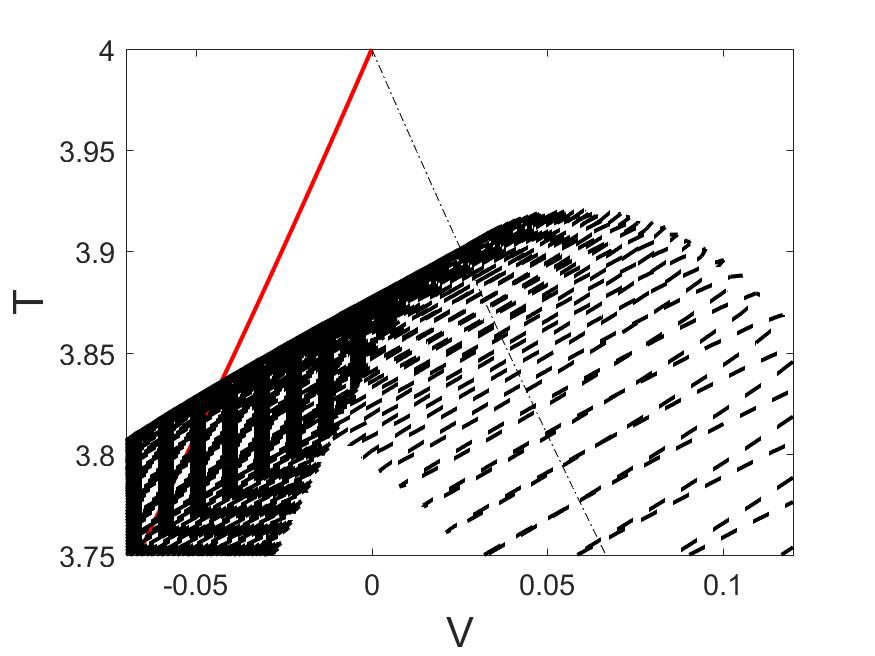
\includegraphics[width=\linewidth]{twoD/slowosc_Tplot_small_zoom.jpg}
  \caption{}
\end{subfigure}
\caption{Model values are $\lambda=.8$, $\epsilon=.01$ with $A=B=2$. In (a) we have the numerical solution (black dotted) over the static equilibrium plot for $V$ vs. $T$. In (b) a zoom of the bifurcation area.}
\label{fig:twoD_slowosc_Tnumerics_small}
\end{figure}

In figure~\ref{fig:twoD_slowosc_Vnumerics_medium} we have chosen a value of $\lambda$ in Case II as $\lambda>1$ but this choice is close to 1. Thus we see comparable behavior to Case I with the addition that the slow variation is now dominant. Upon a zoom in, it is apparent that oscillations are still present and we see the mixture of effects that cause a similar tipping to Case I to take place. We've plotted the tipping point for the slowly varying model \eqref{eq:twoD_slow_tipping} as the green vertical dotted line for comparison. As the numerical tipping point is moving towards the slowly varying tipping point this confirms that the slow variation is indeed dominating the tipping. In figure~\ref{fig:twoD_slowosc_Tnumerics_medium} we again see very similar behavior to the slowly varying model in \autoref{sec:twoD_slow} but the zoom in further reveals the oscillations are present and have minor influence by forcing the solution to cross the $V=0$ axis near the tipping.

\begin{figure}[H]
\centering
\begin{subfigure}{.5\textwidth}
  \centering
  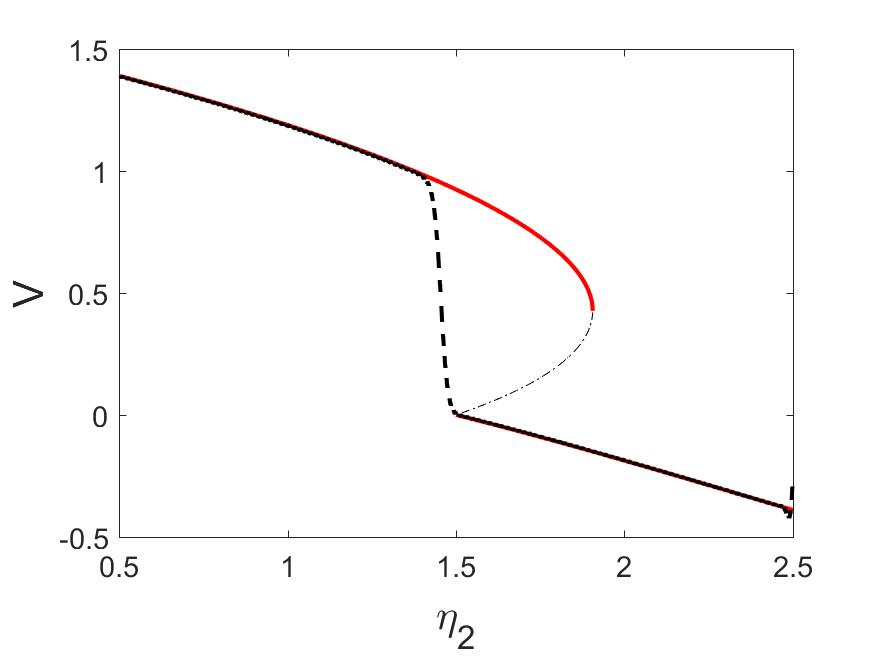
\includegraphics[width=\linewidth]{twoD/slowosc_bif_diagram_medium.jpg}
  \caption{}
\end{subfigure}%
\begin{subfigure}{.5\textwidth}
  \centering
  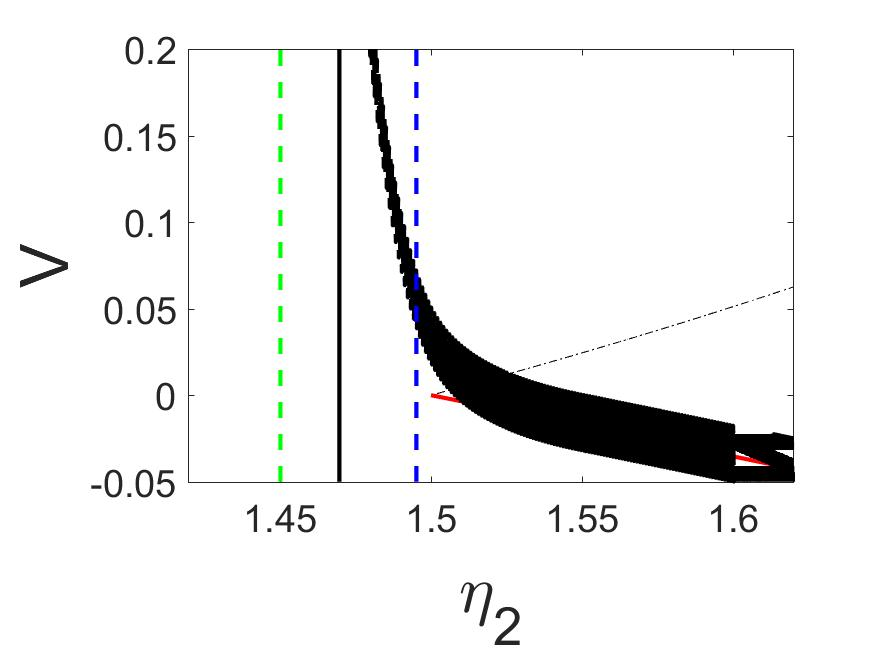
\includegraphics[width=\linewidth]{twoD/slowosc_bif_diagram_medium_zoom.jpg}
  \caption{}
\end{subfigure}
\caption{Model values are $\lambda=1.05$, $\epsilon=.01$ with $A=B=2$. In (a) the numerical solution (black dotted line) to \eqref{eq:twoD_canonical} is given with $\eta_1=4$ and $\eta_3=.375$. In (b) a zoom in closer to the non-smooth bifurcation region where the blue dotted vertical line is the mixed tipping point \eqref{eq:twoD_slowosc_subcaseII_tipping}, green dotted verticle line is the slow tipping point \eqref{eq:twoD_slow_tipping} and the black solid vertical line is the numerically obtained tipping for $V>V_{\text{smooth}}$.}
\label{fig:twoD_slowosc_Vnumerics_medium}
\end{figure}

\begin{figure}[H]
\centering
\begin{subfigure}{.5\textwidth}
  \centering
  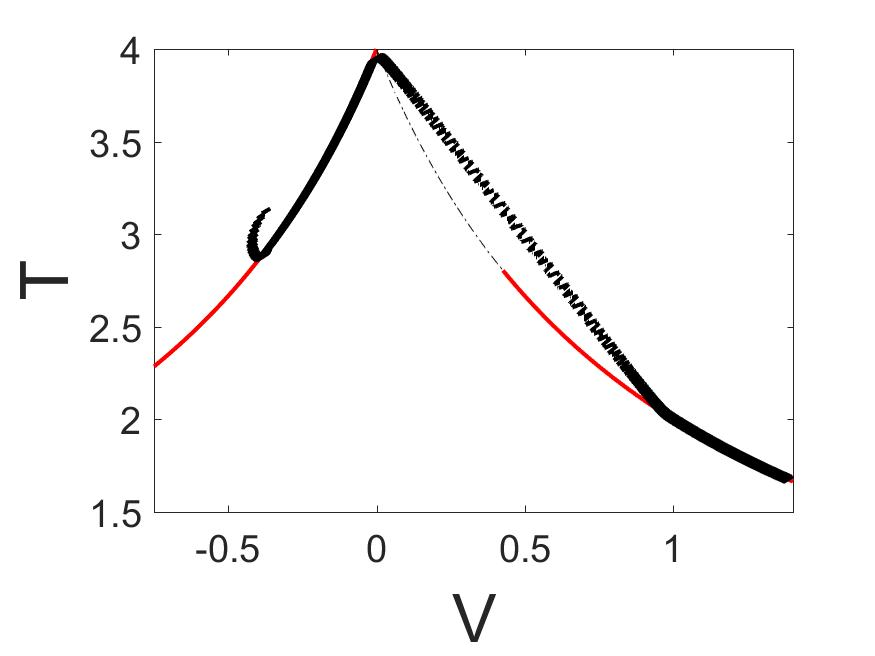
\includegraphics[width=\linewidth]{twoD/slowosc_Tplot_medium.jpg}
  \caption{}
\end{subfigure}%
\begin{subfigure}{.5\textwidth}
  \centering
  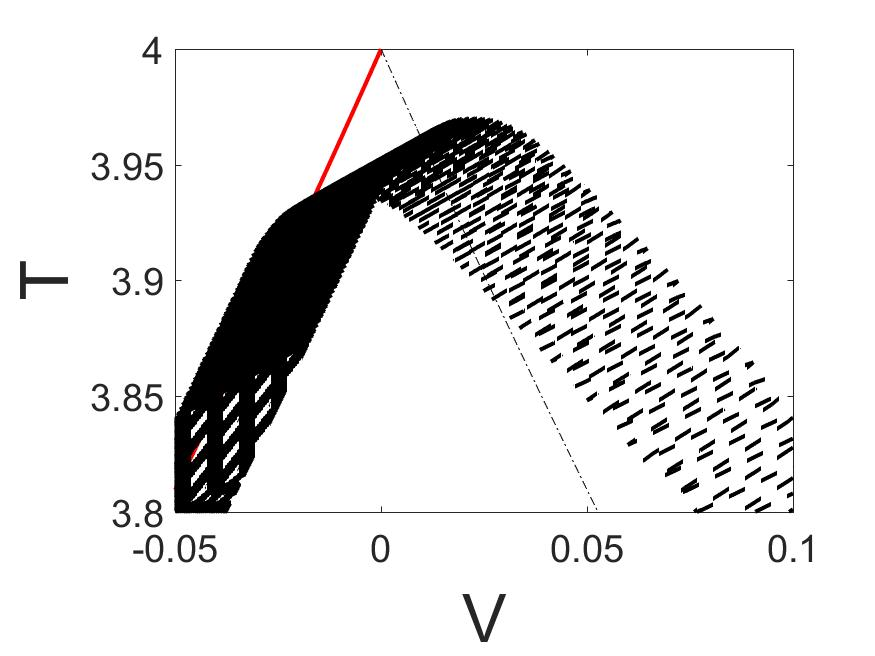
\includegraphics[width=\linewidth]{twoD/slowosc_Tplot_medium_zoom.jpg}
  \caption{}
\end{subfigure}
\caption{Model values are $\lambda=1.05$, $\epsilon=.01$ with $A=B=2$. In (a) we have the numerical solution (black dotted) over the static equilibrium plot for $V$ vs. $T$. In (b) a zoom of the bifurcation area.}
\label{fig:twoD_slowosc_Tnumerics_medium}
\end{figure}

In figure~\ref{fig:twoD_slowosc_Vnumerics_large} we show the numerics for a $\lambda$ large enough so that the oscillations are negligible and we recover the slowly varying model in \autoref{sec:twoD_slow}. Even upon a zoom it is almost impossible to see oscillations in this solution. The green dotted vertical line is the slowly varying tipping estimate \eqref{eq:twoD_slow_tipping} where the blue dotted is the mixed approximation \eqref{eq:twoD_slowosc_subcaseII_tipping}. Further evidence is seen in figure~\ref{fig:twoD_slowosc_Tnumerics_large} where this figure resembles the slowly varying $V-T$ plot \eqref{fig:twoD_slow_Tnumerics}.

\begin{figure}[H]
\centering
\begin{subfigure}{.5\textwidth}
  \centering
  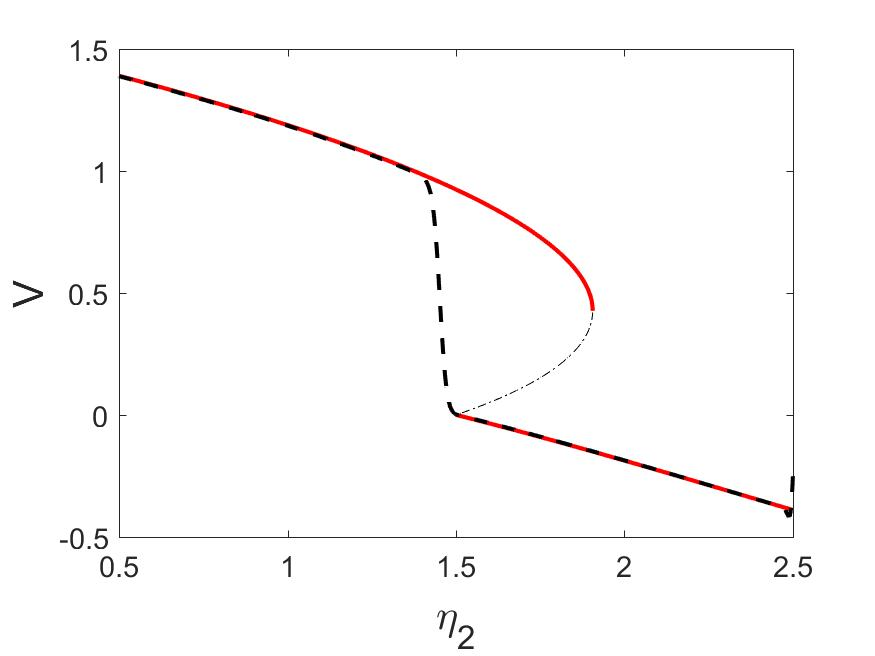
\includegraphics[width=\linewidth]{twoD/slowosc_bif_diagram_large.jpg}
  \caption{}
\end{subfigure}%
\begin{subfigure}{.5\textwidth}
  \centering
  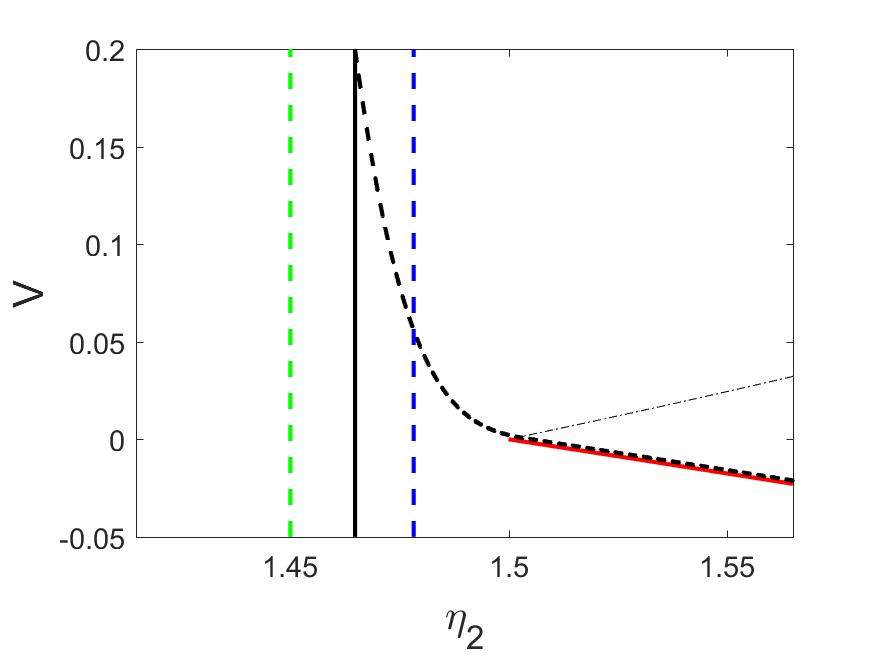
\includegraphics[width=\linewidth]{twoD/slowosc_bif_diagram_large_zoom.jpg}
  \caption{}
\end{subfigure}
\caption{ Model values are $\lambda=2$, $\epsilon=.01$ with $A=B=2$. In (a) the numerical solution (black dotted line) to \eqref{eq:twoD_canonical} is given with $\eta_1=4$ and $\eta_3=.375$. In (b) a zoom in closer to the non-smooth bifurcation region where the blue dotted vertical line is the mixed tipping point \eqref{eq:twoD_slowosc_subcaseII_tipping}, the green dotted vertical line is the slow tipping point \eqref{eq:twoD_slow_tipping} and the black vertical line is the numerically obtained tipping point for $V>V_{\text{smooth}}$.}
\label{fig:twoD_slowosc_Vnumerics_large}
\end{figure}

\begin{figure}[H]
\centering
\begin{subfigure}{.5\textwidth}
  \centering
  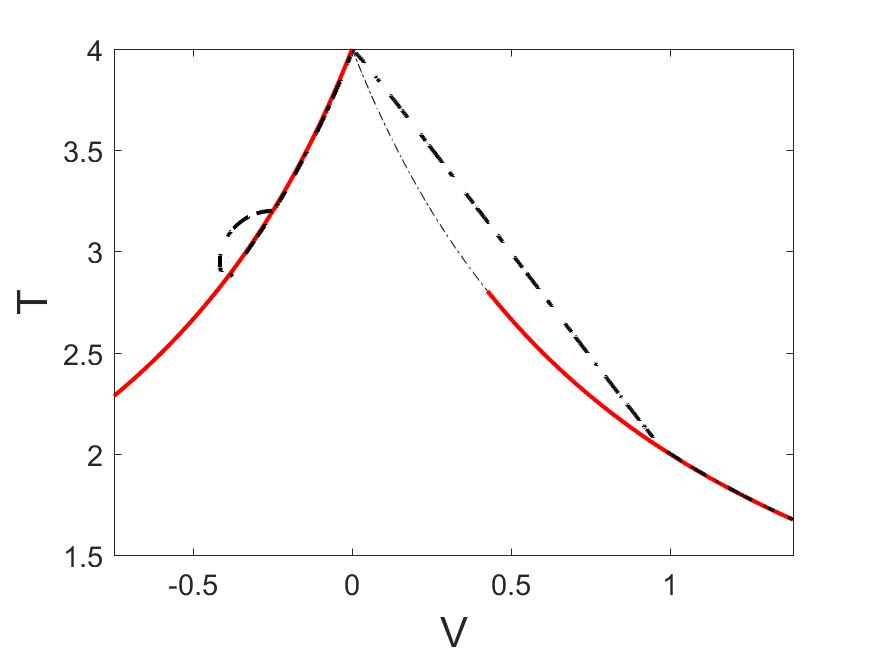
\includegraphics[width=\linewidth]{twoD/slowosc_Tplot_large.jpg}
  \caption{}
\end{subfigure}%
\begin{subfigure}{.5\textwidth}
  \centering
  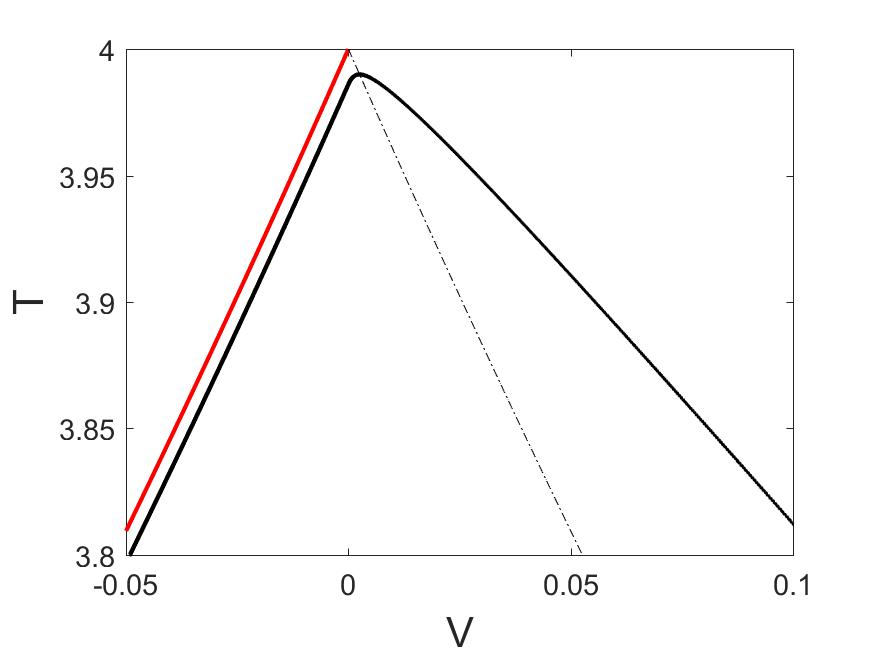
\includegraphics[width=\linewidth]{twoD/slowosc_Tplot_large_zoom.jpg}
  \caption{}
\end{subfigure}
\caption{Model values are $\lambda=2$, $\epsilon=.01$ with $A=B=2$. In (a) we have the numerical solution (black dotted) over the static equilibrium plot for $V$ vs. $T$. In (b) a zoom of the bifurcation area.}
\label{fig:twoD_slowosc_Tnumerics_large}
\end{figure}

Although the figures above show that we have classified the behavior appropriately for the various cases in $\lambda$ and relative solution sizes, performance of our approximate tipping point needs to be evaluated to compare with numerical results. In figure~\ref{fig:twoD_slowosc_lambdacomp} we compare the tipping points between Case I and Case II with the numerically obtained tipping points across a range of $\lambda$ with a fixed $\epsilon$. For smaller $\lambda$, the frequency $\Omega$ is smaller and the influence of the oscillations on tipping become more predominant. But recall the assumption that $\Omega=\epsilon^{-\lambda}\gg 1$ and for $\lambda\le\frac{1}{2}$ we observe $\Omega\sim O(1)$. We do not consider low frequency corresponding to $\lambda<\frac{1}{2}$ in this section. For larger $\lambda$ becomes, there is a reduced influence for the oscillatory forcing until it is negligible for some $\lambda>1$. We notice that our reduction tipping approximation for $\lambda<1$ has some bias and this can be attributed the information lost from reducing the full two-dimensional Riccati equations to a one-dimensional model. Although we use a one-dimensional reduced equation to get these approximations, they seem to be performing quite well across all $\lambda$ hence validating the method developed for tipping with varying $\lambda$.

\begin{figure}[H]
\centering
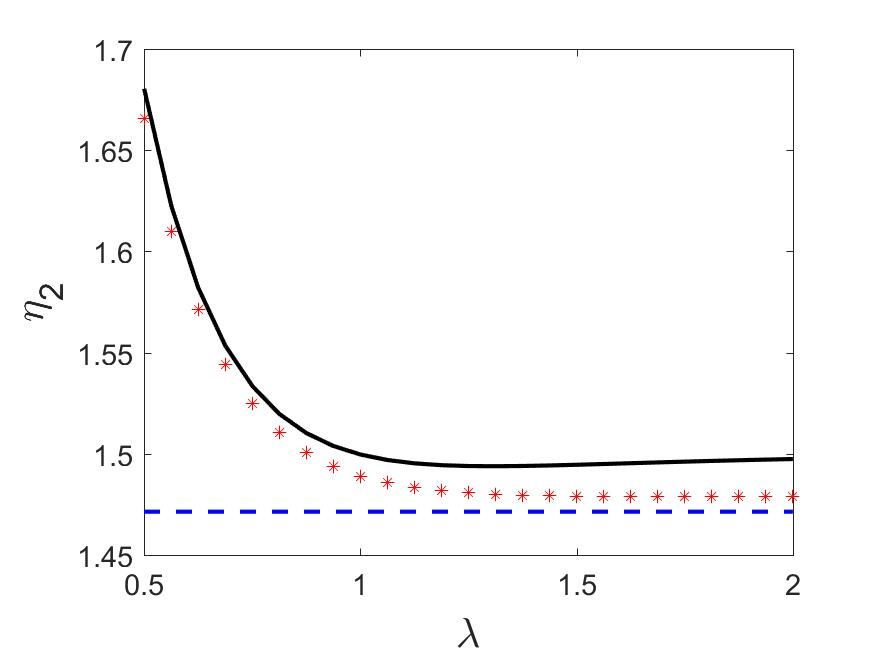
\includegraphics[width=0.7\textwidth]{twoD/slowosc_lambdacomp.jpg}
\caption{An example of numerical tipping (red stars) as the numerical solution to \eqref{eq:oneD_canonical} passes $V>V_{\text{smooth}}$. Parameter values are $\epsilon=.01$ and $A=B=3$. The lines are the Case I tipping estimate (black solid line) and the Case II tipping estimate (blue dotted line).}
\label{fig:twoD_slowosc_lambdacomp}
\end{figure} 

We also are interested in the performance of the tipping approximations across values of $\epsilon$ for $\lambda$ fixed. The performance of each estimate is seen in figure~\ref{fig:twoD_slowosc_epscomp}. For Case I tipping, the range of appropriate $\epsilon$ is highly dependent on the choice in $\lambda$. Often, the range is very small to get accurate estimates. Once this range is left, there are interesting phase effects for the tipping which causes oscillations in the numeric tipping points. For Case II tipping, we that there is a transition happening towards the purely slow tipping, similarly to \autoref{sec:twoD_slow}


\begin{figure}[H]
\centering
\begin{subfigure}{.5\textwidth}
  \centering
  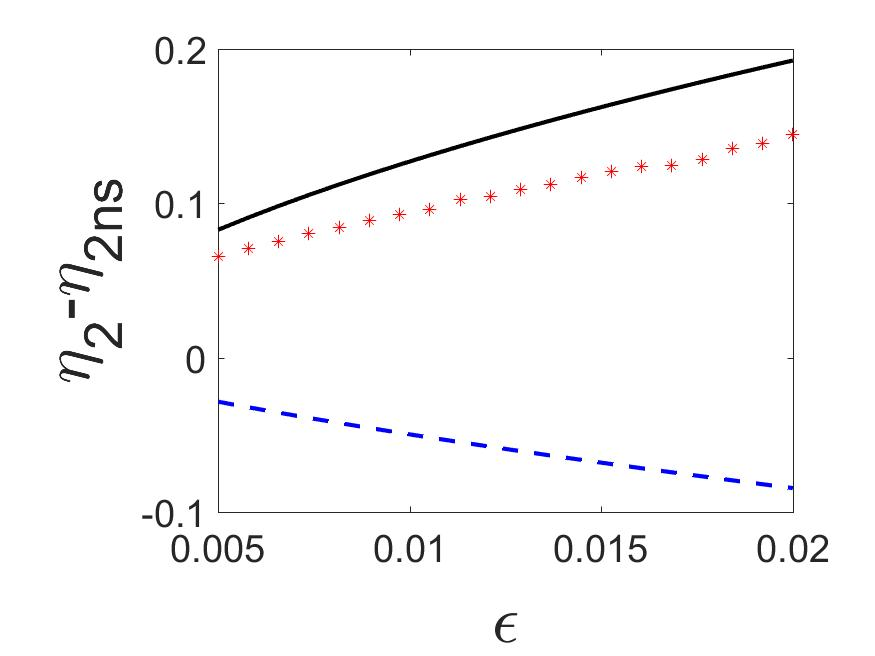
\includegraphics[width=\linewidth]{twoD/slowosc_epscomp_mixed.jpg}
  \caption{$\lambda=.8$}
\end{subfigure}%
\begin{subfigure}{.5\textwidth}
  \centering
  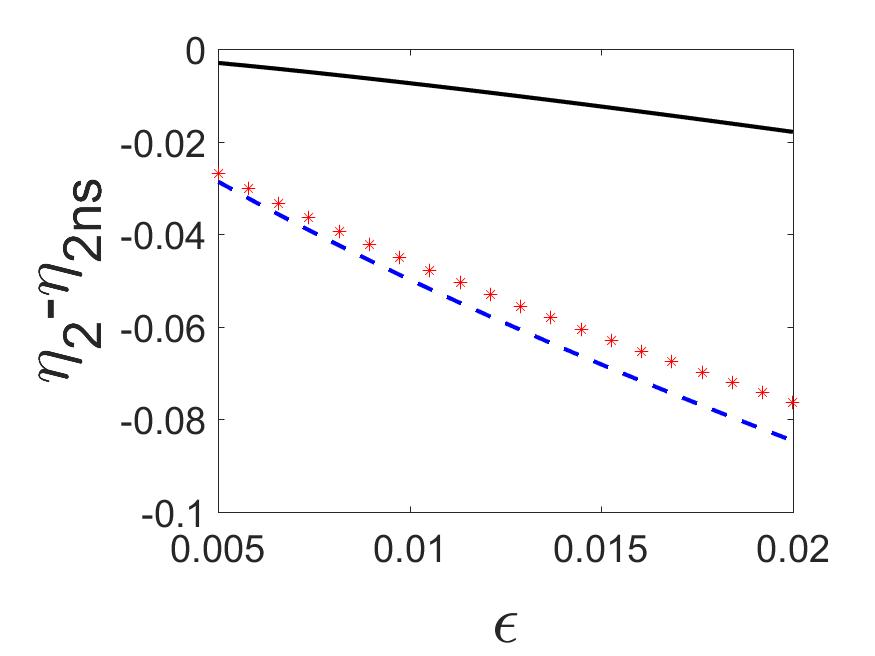
\includegraphics[width=\linewidth]{twoD/slowosc_epscomp_slow.jpg}
  \caption{$\lambda=1.3$}
\end{subfigure}
\caption{The numerical tipping (red stars) follows the appropriate case depending on $\lambda$ for $\epsilon=0.01$. The Case I tipping estimate (black solid line) and purely slow tipping estimate (blue dotted line) are shown.}
\label{fig:twoD_slowosc_epscomp}
\end{figure}

With the numerical results agreeing with our results, we may finally conclude that this method is both useful for analyzing the non-smooth behavior in the Stommel model but also results in an approximation that is more accurate in the extremes of the model (i.e $\Omega \gg 1$ or $\epsilon \ll 1$). This gives us a very accessible means of extracting the tipping in the full two-dimensional without needing to solve difficult Riccati equations or other complex systems that appear from the full problem. All that is needed to verify is our solutions remain stable until we arrive at the region of tipping.

\subsection{Stability}

\subsubsection{Case I: $\lambda\le 1$}

From the analysis, we had discovered the inner equations that govern the behavior of the solution for this range of $\lambda$ are

\begin{equation}\label{eq:twoD_slowosc_stability_caseI_full}
\begin{aligned}
{P_0}_t =& -\epsilon^{1-\lambda} n(t)-\eta_2 P_0 -(1-\eta_3)Q_0,\\
{Q_0}_t =& -\frac{\eta_1}{2\pi}\int_0^{2\pi}|P_0-A\cos(R)|\,dR - Q_0.
\end{aligned}
\end{equation}

But we also found that the relative size of $P_0(t)$ dictates the difficulty of \eqref{eq:twoD_slowosc_stability_caseI_full}. In the analysis we treat these as Sub-Case I: $P_0(t)\le-|A|$ and Sub-Case II: $|P_0(t)|<|A|$ which each require a separate analysis due to their differing behavior.

\subsubsection{Sub-Case I: $P_0(t)\le-|A|$}

We called this the entirely below-axis sub-case due to the solution remaining below the axis and hence predictable under these conditions thus we anticipate this sub-case to remain stable. The equation \eqref{eq:twoD_slowosc_stability_caseI_full} simplifies for this sub-case to

\begin{equation}\label{eq:twoD_slowosc_stability_subcaseI_full}
\begin{aligned}
{P_0}_t =& -\epsilon^{1-\lambda} n(t)-\eta_2 P_0 -(1-\eta_3)Q_0,\\
{Q_0}_t =& \eta_1 P_0 - Q_0.
\end{aligned}
\end{equation}

Which from the analysis we choose to reduce \eqref{eq:twoD_slowosc_stability_subcaseI_full} with the pseudo-equilibria $Q_0(P_0)=\eta_1 P_0$. This gives the following one-dimensional equation with it's pseudo-equilibria as 

\begin{equation}\label{eq:twoD_slowosc_stability_subcaseI_reduced}
\begin{aligned}
{P_0}_t =& -\epsilon^{1-\lambda}n(t)-(\eta_3+\eta_1(1-\eta_3))P_0=f(t,P_0),\\ Z^0(t) =& -\epsilon^{1-\lambda}\frac{n(t)}{\eta_3+\eta_1(1-\eta_3)}.
\end{aligned}
\end{equation}

We adopt a similar strategy for analyzing the stability from the one-dimensional model in \autoref{sec:oneD_slowosc} due to \eqref{eq:twoD_slowosc_stability_subcaseI_reduced} being a one-dimensional equation. Hence we take a simple linear perturbation about the pseudo-equilibrium with $P_0(t)=Z^0(t)+U(t)$ and $\lVert U(t)\rVert \ll 1$. Taking special care to note that $Z^0(t)$ also varies in time, we find the Taylor approximation

\begin{equation}\label{eq:twoD_slowosc_subcaseI_perturb}
\begin{aligned}
{P_0}_t=&f(t,Z^0) +f_{P_0}(t,Z^0)(P_0(t)-Z^0(t))+O(\lVert (P_0(t)-Z^0(t))^2\rVert^2),\\
U_t+Z^0_t =& -(\eta_3+\eta_1(1-\eta_3))U,\\
U_t =& -\epsilon^{1-\lambda}\frac{1}{\eta_3+\eta_1(1-\eta_3)}-(\eta_3+\eta_1(1-\eta_3))U.
\end{aligned}
\end{equation}

With \eqref{eq:twoD_slowosc_subcaseI_perturb} we find that the perturbations decay exponentially to a nearby equilibrium. This indicates the solution for this sub-case is hyperbolically stable and further agrees that no tipping will happen for this size of the solution.

\subsubsection{Sub-Case II: $|P_0(t)|<-|A|$}

We called this the crossing case and from the analysis we anticipate the tipping to occur as the solution is gradually becoming uncontrollable with the crossing. Under the conditions of this sub-case, we integrate \eqref{eq:twoD_slowosc_stability_caseI_full} with the $R_1$ and $R_2$ from the analysis and take the same Taylor approximation to find 

\begin{equation}\label{eq:twoD_slowosc_stability_subcaseII,full}
\begin{aligned}
{P_0}_t =& -n(t)-\eta_3 P_0-(1-\eta_3)Q_0,\\
{Q_0}_t =&-\epsilon^{\lambda-1}\frac{2\eta_1|A|}{\pi}-\epsilon^{1-\lambda}\frac{\eta_1(1-\eta_3)}{\pi|A|}P_0^2-Q_0.
\end{aligned}
\end{equation}

Once more, we assume that the equation for $Q_0$ is in pseudo-equilibrium 
to reduce to the following one-dimensional inner equation with equilibrium where here we let $a=\frac{\eta_1(1-\eta_3)}{\pi|A|}$ for simplicity

\begin{equation}\label{eq:twoD_slowosc_stability_subcaseII,reduced}
\begin{aligned}
{P_0}_t =& -\epsilon^{1-\lambda}n(t)+\frac{2\eta_1(1-\eta_3)|A|}{\pi}-\eta_3 P_0+aP_0^2=f(t,P_0),\\
Z^0(t) =& \frac{1}{2a}\left(\eta_3-\sqrt{4a(\epsilon^{1-\lambda}n(t)-n_{\text{osc}})}\right).
\end{aligned}
\end{equation}

Where we choose to write the argument of the square root in terms of the bifurcation found in \eqref{eq:twoD_osc_bifurcation}. We then consider the linear perturbation about the pseudo-equilibrium $P_0(t)= Z^0(t)+U(t)$ with $\lVert U\rVert \ll 1$. We take a Taylor expansion here to find the dynamics of the perturbation, but recall that we have contributions to the derivative from both the perturbation as well as the pseudo-equilibrium. This is seen with

\begin{equation}
\begin{aligned}
{P_0}_t =& Z^0_t+U_t,\\
Z^0_t=&\begin{cases}
\frac{\epsilon^{1-\lambda}}{\sqrt{4a(\epsilon^{1-\lambda}n(t)-n_{\text{osc}})}} & \epsilon^{1-\lambda}n(t)>n_{\text{osc}},\\
0 & \epsilon^{1-\lambda}n(t)=n_{\text{osc}}.
\end{cases}
\end{aligned}
\end{equation}

Thus we find the following Taylor expansion for the perturbations

\begin{equation}\label{eq:twoD_slowosc_stability_subcaseII_perturb}
\begin{aligned}
{P_0}_t =& f(t,Z^0)+f_{P_0}(t,Z^0)(P_0-Z^0)+O(\lVert P_0-Z^0 \rVert^2),\\
U_t+Z^0_t=& -\sqrt{4a(\epsilon^{1-\lambda}n(t)-n_{\text{osc}})} U,\\
 U_t = & \begin{cases}
\frac{\epsilon^{1-\lambda}}{\sqrt{4a(\epsilon^{1-\lambda}n(t)-n_{\text{osc}})}}-\left(\sqrt{4a(\epsilon^{1-\lambda}n(t)-n_{\text{osc}})}\right) U & \epsilon^{1-\lambda}n(t)>n_{\text{osc}},\\
0 & \epsilon^{1-\lambda}n(t)=n_{\text{osc}}.
\end{cases}
\end{aligned}
\end{equation}

From \eqref{eq:twoD_slowosc_stability_subcaseII_perturb} we find exponentially decaying perturbations that give asymptotic stability until we get to the oscillatory bifurcation. The oscillatory bifurcation corresponds to non-hyperbolic behavior and we lose stability shortly after which indicates of the tipping to occur after the bifurcation.

\subsubsection{Case II: $\lambda>1$}

From the analysis we determined this to be the slowly dominant case and we had discovered the inner equations that govern the behavior of the solution for this range of $\lambda$ to be

\begin{equation}\label{eq:twoD_slowosc_caseII_full}
\begin{aligned}
{P_0}_t =& - n(t)-\eta_2 P_0 -(1-\eta_3)Q_0,\\
{Q_0}_t =& -\frac{\eta_1}{2\pi}\int_0^{2\pi}|P_0-\epsilon^{\lambda-1} A\cos(R)|\,dR - Q_0.
\end{aligned}
\end{equation}

The behavior of this case when $\lambda\sim 1$ is very similar to Case I, thus we anticipate the stability to behave similarly as well. Hence we consider the behavior when $|P_0(t)|<\epsilon^{\lambda-1}|A|$ which is where we found tipping to occur in the analysis. As long as we have $\epsilon^{\lambda-1}A\sim O(1)$, we are follow the same approach as Case I where we integrate \eqref{eq:twoD_slowosc_caseII_full} with a similar $R_1$ and $R_2$ and use a Taylor approximation to get

\begin{equation*}
\begin{aligned}
{P_0}_t =& - n(t)-\eta_2 P_0 -(1-\eta_3)Q_0,\\
{Q_0}_t =& -\epsilon^{\lambda-1}\frac{2\eta_1(1-\eta_3)|A|}{\pi}-\epsilon^{1-\lambda}\frac{\eta_1}{\pi|A|}P_0^2- Q_0.
\end{aligned}
\end{equation*}

The analysis gave sufficient reason to reduce the inner equations to a one-dimensional model and thus like in Case I w find the inner equation with pseudo-equilibrium where here we let $a=\frac{\eta_1(1-\eta_3)}{\pi|A|}$ for simplicity

\begin{equation*}
\begin{aligned}
{P_0}_t =& -n(t)+\epsilon^{\lambda-1}\frac{2\eta_1(1-\eta_3)|A|}{\pi}-\eta_3 P_0+\epsilon^{1-\lambda}aP_0^2,\\
Z^0(t) =& \frac{1}{2a}\left(\epsilon^{\lambda-1}\eta_3-\sqrt{\epsilon^{\lambda-1}4a(n(t)-\epsilon^{\lambda-1}n_{\text{osc}})}\right)
\end{aligned}
\end{equation*}

Where we consider the linear perturbation about the pseudo-equilibrium $P_0(t)= Z^0(t)_U(t)$ with $\lVert U\rVert \ll 1$. We take a Taylor expansion here to find the dynamics of the perturbation, but recall that we have contributions to the derivative from both the perturbation as well as the pseudo-equilibrium. This is seen with

\begin{equation}
\begin{aligned}
{P_0}_t =& Z^0_t+U_t,\\
Z^0_t=&\begin{cases}
\frac{\epsilon^{(\lambda-1)/2}}{\sqrt{4a(n(t)-\epsilon^{\lambda-1}n_{\text{osc}})}} & n(t)>\epsilon^{\lambda-1}n_{\text{osc}},\\
0 & n(t)=\epsilon^{\lambda-1}n_{\text{osc}}.
\end{cases}
\end{aligned}
\end{equation}

Thus we find the following Taylor expansion for the perturbations

\begin{equation}\label{eq:twoD_slowosc_stability_caseII_perturb}
\begin{aligned}
{P_0}_t =& f(t,Z^0)+f_{P_0}(t,Z^0)(P_0-Z^0)+O(\lVert P_0-Z^0 \rVert^2),\\
U_t+Z^0_t=& -\left(\sqrt{\epsilon^{1-\lambda}4a(n(t)-\epsilon^{\lambda-1}n_{\text{osc}})}\right) U,\\
U_t = & \begin{cases}
\frac{\epsilon^{(\lambda-1)/2}}{\sqrt{4a(n(t)-\epsilon^{\lambda-1}n_{\text{osc}})}}-\left(\sqrt{\epsilon^{1-\lambda}4a(n(t)-n_{\text{osc}})}\right) U & n(t)>\epsilon^{\lambda-1}n_{\text{osc}},\\
0 & n(t)=\epsilon^{\lambda-1}n_{\text{osc}}.
\end{cases}
\end{aligned}
\end{equation}

From \eqref{eq:twoD_slowosc_stability_caseII_perturb} we find that the perturbations decay exponentially and we have asymptotic stability until we get to the oscillatory bifurcation. The bifurcation found in \eqref{eq:twoD_osc_bifurcation} corresponds to non-hyperbolic behavior and we then lose the stability which indicates of the tipping to occur after the bifurcation. Comparing this to Case I, we see there is small nuances between these perturbations, although the overall stability remains the same. As for when $\lambda$ grows, we already established this behaves like the purely slow model and hence we can use the stability from that section to conclude that our solution is still stable until the slow tipping point, at which we lose stability as anticipated.


Thus the stability for both Case I and Case II agrees with the results found in the analysis. We have that the behavior of the solution is stable from the outer solution, stability holds before the solution begins to cross the axis $V=0$ and once the crossing begins to happen we lose stability at the location of the oscillatory bifurcation. Because there is slow variation in this model, there is still delayed behavior and thus the tipping happens shorty after the oscillatory bifurcation. In both cases we discovered that the pseudo-equilibrium has a contribution to the derivative and this in turn causes the perturbations to decay towards a small constant. This means that there is a small region around the pseudo-equilibrium that attracts the solution and this is seen in the numerical results. 
